\subsubsection{Core Specification}
\label{sec:corespec}

The remainder of the radial specification is made up of the building blocks 
defined in the previous sections. Specifically, the main core lattice of fuel
assemblies is made up of the previously described fuel assemblies, separated by
the fuel assembly lattice pitch specified in Table
\ref{table_assembly_overview}. In addition, specifications for the structural
components surrounding the fuel assembly lattice are given in Table
\ref{table_baff_vess}.


\begin{table}[htbp]
  \centering
  \caption{Structural component specifications. \label{table_baff_vess}}
  
  \begin{tabularx}{\textwidth}{l C c}
    \toprule
    & & Source \\
    \midrule
    \midrule 
    Baffle Width & 2.22250 cm & \ref{num:core_baffle}\\
    Baffle Water Gap & 0.1627 cm & \ref{num:rpv}\\
    Baffle Material & \hyperlink{mat_SS304}{Stainless Steel 304} & \ref{num:rpv}\\
    
    \\
    Core Barrel \ac{IR} & 187.960 cm & \ref{num:core_barrelIR}\\
    Core Barrel \ac{OR} & 193.675 cm & \ref{num:core_barrelOR}\\
    Core Barrel Material & \hyperlink{mat_SS304}{Stainless Steel 304} & \ref{num:core_barrelmat}\\
    \\
    Neutron Shield Panel \ac{IR} & 194.840 cm & \ref{num:rpv}\\
    Neutron Shield Panel \ac{OR} & 201.630 cm & \ref{num:rpv}\\
    Neutron Shield Panel Material & \hyperlink{mat_SS304}{Stainless Steel 304} & \ref{num:rpv}\\
    Neutron Shield Panel Width & $32^{\circ}$ at the $45^{\circ}$ marks & \ref{num:rpv}\\
    \\
    Pressure Vessel Liner \ac{IR} & 219.150 cm & \ref{num:rpv}\\
    Pressure Vessel Liner \ac{OR} & 219.710 cm & \ref{num:rpv}\\
    Pressure Vessel Liner Material & \hyperlink{mat_SS304}{Stainless Steel 304} & \ref{num:catawba}\\
    \\
    Pressure Vessel \ac{IR} & 219.710 cm & \ref{num:rpv}\\
    Pressure Vessel \ac{OR} & 241.300 cm & \ref{num:rpv}\\
    Pressure Vessel Material & \hyperlink{mat_carbonsteel}{Carbon Steel 508} & \ref{num:catawba}\\
    \bottomrule
  \end{tabularx}

\end{table}

%%%%%%%%%%%%%%%%%%%%%%%%%%%%%%%%%%%%%%%%%%%%%%%%%%%%%%%%%%%%%%%%%%%%%%%%%%%%%%%%
%\FloatBarrier
\paragraph{Enrichment Zones and Burnable Absorber Positions}
\label{sec:corespec_enrba}

The initial cycle 1 fuel assembly loading pattern is shown in Figure
\ref{fig_enr_ba_pos}, including the distribution of enrichments as well as
burnable absorber locations.  The burnable absorber configurations here are
described in Section \ref{sec:ba_configs}, rotated as appropriate for core
symmetry.  A scale view of burnable absorber pins depicting these rotations is
shown in Figure \ref{fig_ba_pos_real}.


\begin{figure}[htbp]
    \centering
    
    % these dimensions are determined in arrow_dimms.ods

    \def\scale{1.0}

    \def\latWidth{0.2673473684*\scale}
    
    \def\RPVOR{3*\scale}
    \def\rectW{0.75*\scale}
    \def\RPVIR{2.7315789474*\scale}
    \def\BarrelIR{2.3368421053*\scale}
    \def\BarrelOR{2.4078947368*\scale}
    \def\ShieldIR{2.4223787816*\scale}
    \def\ShieldOR{2.5067965189*\scale}
    \def\LinerIR{2.7246166598*\scale}

    \def\bafCIRx{0.9357157895*\scale}
    \def\bafCIRy{2.0051052632*\scale}
    \def\bafCORx{0.9633473684*\scale}
    \def\bafCORy{2.0327368421*\scale}
    \def\bafMIRx{1.7377578947*\scale}
    \def\bafMIRy{1.4704105263*\scale}
    \def\bafMORx{1.7653894737*\scale}
    \def\bafMORy{1.4980421053*\scale}
    
    \tikzset{Assembly/.style={
        inner sep=0pt,
        text width=\latWidth in,
        minimum size=\latWidth in,
        draw=black,
        align=center
        }
    }
    
    \def\tkzRPV{(0,0) circle (\RPVIR) (0,0) circle (\RPVOR)}
    \def\tkzLiner{(0,0) circle (\LinerIR) (0,0) circle (\RPVIR)}
    \def\tkzBarrel{(0,0) circle (\BarrelIR) (0,0) circle (\BarrelOR)}
    \def\tkzShields{(0,0) circle (\ShieldIR) (0,0) circle (\ShieldOR)}
    
    \def\tkzBaffCOR{(-\bafCORx, -\bafCORy) rectangle (\bafCORx, \bafCORy)}
    \def\tkzBaffCIR{(-\bafCIRx, -\bafCIRy) rectangle (\bafCIRx, \bafCIRy)} 
    \def\tkzBaffMOR{(-\bafMORx, -\bafMORy) rectangle (\bafMORx, \bafMORy)}
    \def\tkzBaffMIR{(-\bafMIRx, -\bafMIRy) rectangle (\bafMIRx, \bafMIRy) }
    \def\tkzBaffleC{ \tkzBaffCIR \tkzBaffCOR }
    \def\tkzBaffleM{ \tkzBaffMIR \tkzBaffMOR }

    \def\tkzBaffCClip{\tkzBaffCIR (-\RPVOR, -\RPVOR) rectangle (\RPVOR, \RPVOR)}
    \def\tkzBaffMClip{\tkzBaffMIR (-\RPVOR, -\RPVOR) rectangle (\RPVOR, \RPVOR)}

    \def\highenr{blue!50}
    \def\midenr{yellow!50}
    \def\lowenr{red!50}

    \scalebox{1.0}{

      \begin{tikzpicture}[x=1in,y=1in]
      
        % draw RPV, barrel, liner and shield panels
        
        \path[fill=black!90!white,even odd rule] \tkzRPV;
        \path[fill=black,even odd rule] \tkzLiner;
        \path[fill=black,even odd rule] \tkzBarrel;
        \begin{scope}
          \clip (0,0) -- +(61:\RPVOR) arc (61:29:\RPVOR) --
                (0,0) -- +(151:\RPVOR) arc (151:119:\RPVOR) -- 
                (0,0) -- +(241:\RPVOR) arc (241:209:\RPVOR) -- 
                (0,0) -- +(331:\RPVOR) arc (331:299:\RPVOR) -- cycle;
          \path[fill=black,even odd rule] \tkzShields;
        \end{scope}

        % draw baffle north/south
        
        \begin{scope}[even odd rule]
          \clip[rotate=90] \tkzBaffMClip;
          \path[fill=black] \tkzBaffleC;
        \end{scope}
        \begin{scope}[even odd rule]
          \clip \tkzBaffCClip;
          \clip \tkzBaffMClip;
          \path[fill=black, rotate=90] \tkzBaffleM;
        \end{scope}
        
        % draw baffle east/west
        
        \begin{scope}[rotate=90]
          \begin{scope}[even odd rule]
            \clip[rotate=90] \tkzBaffMClip;
            \path[fill=black] \tkzBaffleC;
          \end{scope}
          \begin{scope}[even odd rule]
            \clip \tkzBaffCClip;
            \clip \tkzBaffMClip;
            \path[fill=black, rotate=90] \tkzBaffleM;
          \end{scope}
        \end{scope}
        
        % draw assembly row/column headers
        
        \draw[red, thick] ($(-7*\latWidth,\RPVOR/\latWidth*\latWidth)$) node[above, anchor=south] {R} -- ($(-7*\latWidth,4*\latWidth)$);
        \draw[red, thick] ($(-6*\latWidth,\RPVOR/\latWidth*\latWidth)$) node[above, anchor=south] {P} -- ($(-6*\latWidth,6*\latWidth)$);
        \draw[red, thick] ($(-5*\latWidth,\RPVOR/\latWidth*\latWidth)$) node[above, anchor=south] {N} -- ($(-5*\latWidth,7*\latWidth)$);
        \draw[red, thick] ($(-4*\latWidth,\RPVOR/\latWidth*\latWidth)$) node[above, anchor=south] {M} -- ($(-4*\latWidth,7*\latWidth)$);
        \draw[red, thick] ($(-3*\latWidth,\RPVOR/\latWidth*\latWidth)$) node[above, anchor=south] {L} -- ($(-3*\latWidth,8*\latWidth)$);
        \draw[red, thick] ($(-2*\latWidth,\RPVOR/\latWidth*\latWidth)$) node[above, anchor=south] {K} -- ($(-2*\latWidth,8*\latWidth)$);
        \draw[red, thick] ($(-1*\latWidth,\RPVOR/\latWidth*\latWidth)$) node[above, anchor=south] {J} -- ($(-1*\latWidth,8*\latWidth)$);
        \draw[red, thick] ($(-0*\latWidth,\RPVOR/\latWidth*\latWidth)$) node[above, anchor=south] {H} -- ($(-0*\latWidth,8*\latWidth)$);
        \draw[red, thick] ($(1*\latWidth,\RPVOR/\latWidth*\latWidth)$) node[above, anchor=south] {G} -- ($(1*\latWidth,8*\latWidth)$);
        \draw[red, thick] ($(2*\latWidth,\RPVOR/\latWidth*\latWidth)$) node[above, anchor=south] {F} -- ($(2*\latWidth,8*\latWidth)$);
        \draw[red, thick] ($(3*\latWidth,\RPVOR/\latWidth*\latWidth)$) node[above, anchor=south] {E} -- ($(3*\latWidth,8*\latWidth)$);
        \draw[red, thick] ($(4*\latWidth,\RPVOR/\latWidth*\latWidth)$) node[above, anchor=south] {D} -- ($(4*\latWidth,7*\latWidth)$);
        \draw[red, thick] ($(5*\latWidth,\RPVOR/\latWidth*\latWidth)$) node[above, anchor=south] {C} -- ($(5*\latWidth,7*\latWidth)$);
        \draw[red, thick] ($(6*\latWidth,\RPVOR/\latWidth*\latWidth)$) node[above, anchor=south] {B} -- ($(6*\latWidth,6*\latWidth)$);
        \draw[red, thick] ($(7*\latWidth,\RPVOR/\latWidth*\latWidth)$) node[above, anchor=south] {A} -- ($(7*\latWidth,4*\latWidth)$);
        
        \begin{scope}[rotate=90]
          \draw[red, thick] ($(-7*\latWidth,\RPVOR/\latWidth*\latWidth)$) node[left, anchor=east] {15} -- ($(-7*\latWidth,4*\latWidth)$);
          \draw[red, thick] ($(-6*\latWidth,\RPVOR/\latWidth*\latWidth)$) node[left, anchor=east] {14} -- ($(-6*\latWidth,6*\latWidth)$);
          \draw[red, thick] ($(-5*\latWidth,\RPVOR/\latWidth*\latWidth)$) node[left, anchor=east] {13} -- ($(-5*\latWidth,7*\latWidth)$);
          \draw[red, thick] ($(-4*\latWidth,\RPVOR/\latWidth*\latWidth)$) node[left, anchor=east] {12} -- ($(-4*\latWidth,7*\latWidth)$);
          \draw[red, thick] ($(-3*\latWidth,\RPVOR/\latWidth*\latWidth)$) node[left, anchor=east] {11} -- ($(-3*\latWidth,8*\latWidth)$);
          \draw[red, thick] ($(-2*\latWidth,\RPVOR/\latWidth*\latWidth)$) node[left, anchor=east] {10} -- ($(-2*\latWidth,8*\latWidth)$);
          \draw[red, thick] ($(-1*\latWidth,\RPVOR/\latWidth*\latWidth)$) node[left, anchor=east] {9} -- ($(-1*\latWidth,8*\latWidth)$);
          \draw[red, thick] ($(-0*\latWidth,\RPVOR/\latWidth*\latWidth)$) node[left, anchor=east] {8} -- ($(-0*\latWidth,8*\latWidth)$);
          \draw[red, thick] ($(1*\latWidth,\RPVOR/\latWidth*\latWidth)$) node[left, anchor=east] {7} -- ($(1*\latWidth,8*\latWidth)$);
          \draw[red, thick] ($(2*\latWidth,\RPVOR/\latWidth*\latWidth)$) node[left, anchor=east] {6} -- ($(2*\latWidth,8*\latWidth)$);
          \draw[red, thick] ($(3*\latWidth,\RPVOR/\latWidth*\latWidth)$) node[left, anchor=east] {5} -- ($(3*\latWidth,8*\latWidth)$);
          \draw[red, thick] ($(4*\latWidth,\RPVOR/\latWidth*\latWidth)$) node[left, anchor=east] {4} -- ($(4*\latWidth,7*\latWidth)$);
          \draw[red, thick] ($(5*\latWidth,\RPVOR/\latWidth*\latWidth)$) node[left, anchor=east] {3} -- ($(5*\latWidth,7*\latWidth)$);
          \draw[red, thick] ($(6*\latWidth,\RPVOR/\latWidth*\latWidth)$) node[left, anchor=east] {2} -- ($(6*\latWidth,6*\latWidth)$);
          \draw[red, thick] ($(7*\latWidth,\RPVOR/\latWidth*\latWidth)$) node[left, anchor=east] {1} -- ($(7*\latWidth,4*\latWidth)$);
        \end{scope}
        
        % draw fuel assembly nodes
        
        \node [Assembly, fill=\highenr] at ($(-3*\latWidth,7*\latWidth)$) {}; % L1
        \node [Assembly, fill=\highenr, hyperlink node=ass_6ba_target] at ($(-2*\latWidth,7*\latWidth)$) {6}; % K1
        \node [Assembly, fill=\highenr] at ($(-1*\latWidth,7*\latWidth)$) {}; % J1
        \node [Assembly, fill=\highenr, hyperlink node=ass_6ba_target] at ($(-0*\latWidth,7*\latWidth)$) {6}; % H1
        \node [Assembly, fill=\highenr] at ($( 1*\latWidth,7*\latWidth)$) {}; % G1
        \node [Assembly, fill=\highenr, hyperlink node=ass_6ba_target] at ($( 2*\latWidth,7*\latWidth)$) {6}; % F1
        \node [Assembly, fill=\highenr] at ($( 3*\latWidth,7*\latWidth)$) {}; % E1

        \node [Assembly, fill=\highenr] at ($(-5*\latWidth,6*\latWidth)$) {}; % N2
        \node [Assembly, fill=\highenr] at ($(-4*\latWidth,6*\latWidth)$) {}; % M2
        \node [Assembly, fill=\highenr, hyperlink node=ass_16ba_target] at ($(-3*\latWidth,6*\latWidth)$) {16}; % L2
        \node [Assembly, fill=\lowenr] at ($(-2*\latWidth,6*\latWidth)$) {}; % K2
        \node [Assembly, fill=\highenr, hyperlink node=ass_20ba_target] at ($(-1*\latWidth,6*\latWidth)$) {20}; % J2
        \node [Assembly, fill=\lowenr] at ($(-0*\latWidth,6*\latWidth)$) {}; % H2
        \node [Assembly, fill=\highenr, hyperlink node=ass_20ba_target] at ($( 1*\latWidth,6*\latWidth)$) {20}; % G2
        \node [Assembly, fill=\lowenr] at ($( 2*\latWidth,6*\latWidth)$) {}; % F2
        \node [Assembly, fill=\highenr, hyperlink node=ass_16ba_target] at ($( 3*\latWidth,6*\latWidth)$) {16}; % E2
        \node [Assembly, fill=\highenr] at ($( 4*\latWidth,6*\latWidth)$) {}; % D2
        \node [Assembly, fill=\highenr] at ($( 5*\latWidth,6*\latWidth)$) {}; % C2

        \node [Assembly, fill=\highenr] at ($(-6*\latWidth,5*\latWidth)$) {}; % P3
        \node [Assembly, fill=\highenr, hyperlink node=ass_15ba_target] at ($(-5*\latWidth,5*\latWidth)$) {15}; % N3
        \node [Assembly, fill=\midenr, hyperlink node=ass_16ba_target] at ($(-4*\latWidth,5*\latWidth)$) {16}; % M3
        \node [Assembly, fill=\lowenr] at ($(-3*\latWidth,5*\latWidth)$) {}; % L3
        \node [Assembly, fill=\midenr, hyperlink node=ass_16ba_target] at ($(-2*\latWidth,5*\latWidth)$) {16}; % K3
        \node [Assembly, fill=\lowenr] at ($(-1*\latWidth,5*\latWidth)$) {}; % J3
        \node [Assembly, fill=\midenr, hyperlink node=ass_16ba_target] at ($(-0*\latWidth,5*\latWidth)$) {16}; % H3
        \node [Assembly, fill=\lowenr] at ($( 1*\latWidth,5*\latWidth)$) {}; % G3
        \node [Assembly, fill=\midenr, hyperlink node=ass_16ba_target] at ($( 2*\latWidth,5*\latWidth)$) {16}; % F3
        \node [Assembly, fill=\lowenr] at ($( 3*\latWidth,5*\latWidth)$) {}; % E3
        \node [Assembly, fill=\midenr, hyperlink node=ass_16ba_target] at ($( 4*\latWidth,5*\latWidth)$) {16}; % D3
        \node [Assembly, fill=\highenr, hyperlink node=ass_15ba_target] at ($( 5*\latWidth,5*\latWidth)$) {15}; % C3
        \node [Assembly, fill=\highenr] at ($( 6*\latWidth,5*\latWidth)$) {}; % B3

        \node [Assembly, fill=\highenr] at ($(-6*\latWidth,4*\latWidth)$) {}; % P4
        \node [Assembly, fill=\midenr, hyperlink node=ass_16ba_target] at ($(-5*\latWidth,4*\latWidth)$) {16}; % N4
        \node [Assembly, fill=\midenr] at ($(-4*\latWidth,4*\latWidth)$) {}; % M4
        \node [Assembly, fill=\midenr, hyperlink node=ass_16ba_target] at ($(-3*\latWidth,4*\latWidth)$) {16}; % L4
        \node [Assembly, fill=\lowenr] at ($(-2*\latWidth,4*\latWidth)$) {}; % K4
        \node [Assembly, fill=\midenr, hyperlink node=ass_12ba_target] at ($(-1*\latWidth,4*\latWidth)$) {12}; % J4
        \node [Assembly, fill=\lowenr] at ($(-0*\latWidth,4*\latWidth)$) {}; % H4
        \node [Assembly, fill=\midenr, hyperlink node=ass_12ba_target] at ($( 1*\latWidth,4*\latWidth)$) {12}; % G4
        \node [Assembly, fill=\lowenr] at ($( 2*\latWidth,4*\latWidth)$) {}; % F4
        \node [Assembly, fill=\midenr, hyperlink node=ass_16ba_target] at ($( 3*\latWidth,4*\latWidth)$) {16}; % E4
        \node [Assembly, fill=\midenr] at ($( 4*\latWidth,4*\latWidth)$) {}; % D4
        \node [Assembly, fill=\midenr, hyperlink node=ass_16ba_target] at ($( 5*\latWidth,4*\latWidth)$) {16}; % C4
        \node [Assembly, fill=\highenr] at ($( 6*\latWidth,4*\latWidth)$) {}; % B4

        \node [Assembly, fill=\highenr] at ($(-7*\latWidth,3*\latWidth)$) {}; % R5
        \node [Assembly, fill=\highenr, hyperlink node=ass_16ba_target] at ($(-6*\latWidth,3*\latWidth)$) {16}; % P5
        \node [Assembly, fill=\lowenr] at ($(-5*\latWidth,3*\latWidth)$) {}; % N5
        \node [Assembly, fill=\midenr, hyperlink node=ass_16ba_target] at ($(-4*\latWidth,3*\latWidth)$) {16}; % M5
        \node [Assembly, fill=\lowenr] at ($(-3*\latWidth,3*\latWidth)$) {}; % L5
        \node [Assembly, fill=\midenr, hyperlink node=ass_12ba_target] at ($(-2*\latWidth,3*\latWidth)$) {12}; % K5
        \node [Assembly, fill=\lowenr] at ($(-1*\latWidth,3*\latWidth)$) {}; % J5
        \node [Assembly, fill=\midenr, hyperlink node=ass_12ba_target] at ($(-0*\latWidth,3*\latWidth)$) {12}; % H5
        \node [Assembly, fill=\lowenr] at ($( 1*\latWidth,3*\latWidth)$) {}; % G5
        \node [Assembly, fill=\midenr, hyperlink node=ass_12ba_target] at ($( 2*\latWidth,3*\latWidth)$) {12}; % F5
        \node [Assembly, fill=\lowenr] at ($( 3*\latWidth,3*\latWidth)$) {}; % E5
        \node [Assembly, fill=\midenr, hyperlink node=ass_16ba_target] at ($( 4*\latWidth,3*\latWidth)$) {16}; % D5
        \node [Assembly, fill=\lowenr] at ($( 5*\latWidth,3*\latWidth)$) {}; % C5
        \node [Assembly, fill=\highenr, hyperlink node=ass_16ba_target] at ($( 6*\latWidth,3*\latWidth)$) {16}; % B5
        \node [Assembly, fill=\highenr] at ($( 7*\latWidth,3*\latWidth)$) {}; % A5

        \node [Assembly, fill=\highenr, hyperlink node=ass_6ba_target] at ($(-7*\latWidth,2*\latWidth)$) {6}; % R6
        \node [Assembly, fill=\lowenr] at ($(-6*\latWidth,2*\latWidth)$) {}; % P6
        \node [Assembly, fill=\midenr, hyperlink node=ass_16ba_target] at ($(-5*\latWidth,2*\latWidth)$) {16}; % N6
        \node [Assembly, fill=\lowenr] at ($(-4*\latWidth,2*\latWidth)$) {}; % M6
        \node [Assembly, fill=\midenr, hyperlink node=ass_12ba_target] at ($(-3*\latWidth,2*\latWidth)$) {12}; % L6
        \node [Assembly, fill=\lowenr] at ($(-2*\latWidth,2*\latWidth)$) {}; % K6
        \node [Assembly, fill=\midenr, hyperlink node=ass_12ba_target] at ($(-1*\latWidth,2*\latWidth)$) {12}; % J6
        \node [Assembly, fill=\lowenr] at ($(-0*\latWidth,2*\latWidth)$) {}; % H6
        \node [Assembly, fill=\midenr, hyperlink node=ass_12ba_target] at ($( 1*\latWidth,2*\latWidth)$) {12}; % G6
        \node [Assembly, fill=\lowenr] at ($( 2*\latWidth,2*\latWidth)$) {}; % F6
        \node [Assembly, fill=\midenr, hyperlink node=ass_12ba_target] at ($( 3*\latWidth,2*\latWidth)$) {12}; % E6
        \node [Assembly, fill=\lowenr] at ($( 4*\latWidth,2*\latWidth)$) {}; % D6
        \node [Assembly, fill=\midenr, hyperlink node=ass_16ba_target] at ($( 5*\latWidth,2*\latWidth)$) {16}; % C6
        \node [Assembly, fill=\lowenr] at ($( 6*\latWidth,2*\latWidth)$) {}; % B6
        \node [Assembly, fill=\highenr, hyperlink node=ass_6ba_target] at ($( 7*\latWidth,2*\latWidth)$) {6}; % A6

        \node [Assembly, fill=\highenr] at ($(-7*\latWidth,1*\latWidth)$) {}; % R7
        \node [Assembly, fill=\highenr, hyperlink node=ass_20ba_target] at ($(-6*\latWidth,1*\latWidth)$) {20}; % P7
        \node [Assembly, fill=\lowenr] at ($(-5*\latWidth,1*\latWidth)$) {}; % N7
        \node [Assembly, fill=\midenr, hyperlink node=ass_12ba_target] at ($(-4*\latWidth,1*\latWidth)$) {12}; % M7
        \node [Assembly, fill=\lowenr] at ($(-3*\latWidth,1*\latWidth)$) {}; % L7
        \node [Assembly, fill=\midenr, hyperlink node=ass_12ba_target] at ($(-2*\latWidth,1*\latWidth)$) {12}; % K7
        \node [Assembly, fill=\lowenr] at ($(-1*\latWidth,1*\latWidth)$) {}; % J7
        \node [Assembly, fill=\midenr, hyperlink node=ass_16ba_target] at ($(-0*\latWidth,1*\latWidth)$) {16}; % H7
        \node [Assembly, fill=\lowenr] at ($( 1*\latWidth,1*\latWidth)$) {}; % G7
        \node [Assembly, fill=\midenr, hyperlink node=ass_12ba_target] at ($( 2*\latWidth,1*\latWidth)$) {12}; % F7
        \node [Assembly, fill=\lowenr] at ($( 3*\latWidth,1*\latWidth)$) {}; % E7
        \node [Assembly, fill=\midenr, hyperlink node=ass_12ba_target] at ($( 4*\latWidth,1*\latWidth)$) {12}; % D7
        \node [Assembly, fill=\lowenr] at ($( 5*\latWidth,1*\latWidth)$) {}; % C7
        \node [Assembly, fill=\highenr, hyperlink node=ass_20ba_target] at ($( 6*\latWidth,1*\latWidth)$) {20}; % B7
        \node [Assembly, fill=\highenr] at ($( 7*\latWidth,1*\latWidth)$) {}; % A7

        \node [Assembly, fill=\highenr, hyperlink node=ass_6ba_target] at ($(-7*\latWidth,0*\latWidth)$) {6}; % R8
        \node [Assembly, fill=\lowenr] at ($(-6*\latWidth,0*\latWidth)$) {}; % P8
        \node [Assembly, fill=\midenr, hyperlink node=ass_16ba_target] at ($(-5*\latWidth,0*\latWidth)$) {16}; % N8
        \node [Assembly, fill=\lowenr] at ($(-4*\latWidth,0*\latWidth)$) {}; % M8
        \node [Assembly, fill=\midenr, hyperlink node=ass_12ba_target] at ($(-3*\latWidth,0*\latWidth)$) {12}; % L8
        \node [Assembly, fill=\lowenr] at ($(-2*\latWidth,0*\latWidth)$) {}; % K8
        \node [Assembly, fill=\midenr, hyperlink node=ass_16ba_target] at ($(-1*\latWidth,0*\latWidth)$) {16}; % J8
        \node [Assembly, fill=\lowenr] at ($(-0*\latWidth,0*\latWidth)$) {}; % H8
        \node [Assembly, fill=\midenr, hyperlink node=ass_16ba_target] at ($( 1*\latWidth,0*\latWidth)$) {16}; % G8
        \node [Assembly, fill=\lowenr] at ($( 2*\latWidth,0*\latWidth)$) {}; % F8
        \node [Assembly, fill=\midenr, hyperlink node=ass_12ba_target] at ($( 3*\latWidth,0*\latWidth)$) {12}; % E8
        \node [Assembly, fill=\lowenr] at ($( 4*\latWidth,0*\latWidth)$) {}; % D8
        \node [Assembly, fill=\midenr, hyperlink node=ass_16ba_target] at ($( 5*\latWidth,0*\latWidth)$) {16}; % C8
        \node [Assembly, fill=\lowenr] at ($( 6*\latWidth,0*\latWidth)$) {}; % B8
        \node [Assembly, fill=\highenr, hyperlink node=ass_6ba_target] at ($( 7*\latWidth,0*\latWidth)$) {6}; % A8

        \node [Assembly, fill=\highenr] at ($(-7*\latWidth,-1*\latWidth)$) {}; % R9
        \node [Assembly, fill=\highenr, hyperlink node=ass_20ba_target] at ($(-6*\latWidth,-1*\latWidth)$) {20}; % P9
        \node [Assembly, fill=\lowenr] at ($(-5*\latWidth,-1*\latWidth)$) {}; % N9
        \node [Assembly, fill=\midenr, hyperlink node=ass_12ba_target] at ($(-4*\latWidth,-1*\latWidth)$) {12}; % M9
        \node [Assembly, fill=\lowenr] at ($(-3*\latWidth,-1*\latWidth)$) {}; % L9
        \node [Assembly, fill=\midenr, hyperlink node=ass_12ba_target] at ($(-2*\latWidth,-1*\latWidth)$) {12}; % K9
        \node [Assembly, fill=\lowenr] at ($(-1*\latWidth,-1*\latWidth)$) {}; % J9
        \node [Assembly, fill=\midenr, hyperlink node=ass_16ba_target] at ($(-0*\latWidth,-1*\latWidth)$) {16}; % H9
        \node [Assembly, fill=\lowenr] at ($( 1*\latWidth,-1*\latWidth)$) {}; % G9
        \node [Assembly, fill=\midenr, hyperlink node=ass_12ba_target] at ($( 2*\latWidth,-1*\latWidth)$) {12}; % F9
        \node [Assembly, fill=\lowenr] at ($( 3*\latWidth,-1*\latWidth)$) {}; % E9
        \node [Assembly, fill=\midenr, hyperlink node=ass_12ba_target] at ($( 4*\latWidth,-1*\latWidth)$) {12}; % D9
        \node [Assembly, fill=\lowenr] at ($( 5*\latWidth,-1*\latWidth)$) {}; % C9
        \node [Assembly, fill=\highenr, hyperlink node=ass_20ba_target] at ($( 6*\latWidth,-1*\latWidth)$) {20}; % B9
        \node [Assembly, fill=\highenr] at ($( 7*\latWidth,-1*\latWidth)$) {}; % A9

        \node [Assembly, fill=\highenr, hyperlink node=ass_6ba_target] at ($(-7*\latWidth,-2*\latWidth)$) {6}; % R10
        \node [Assembly, fill=\lowenr] at ($(-6*\latWidth,-2*\latWidth)$) {}; % P10
        \node [Assembly, fill=\midenr, hyperlink node=ass_16ba_target] at ($(-5*\latWidth,-2*\latWidth)$) {16}; % N10
        \node [Assembly, fill=\lowenr] at ($(-4*\latWidth,-2*\latWidth)$) {}; % M10
        \node [Assembly, fill=\midenr, hyperlink node=ass_12ba_target] at ($(-3*\latWidth,-2*\latWidth)$) {12}; % L10
        \node [Assembly, fill=\lowenr] at ($(-2*\latWidth,-2*\latWidth)$) {}; % K10
        \node [Assembly, fill=\midenr, hyperlink node=ass_12ba_target] at ($(-1*\latWidth,-2*\latWidth)$) {12}; % J10
        \node [Assembly, fill=\lowenr] at ($(-0*\latWidth,-2*\latWidth)$) {}; % H10
        \node [Assembly, fill=\midenr, hyperlink node=ass_12ba_target] at ($( 1*\latWidth,-2*\latWidth)$) {12}; % G10
        \node [Assembly, fill=\lowenr] at ($( 2*\latWidth,-2*\latWidth)$) {}; % F10
        \node [Assembly, fill=\midenr, hyperlink node=ass_12ba_target] at ($( 3*\latWidth,-2*\latWidth)$) {12}; % E10
        \node [Assembly, fill=\lowenr] at ($( 4*\latWidth,-2*\latWidth)$) {}; % D10
        \node [Assembly, fill=\midenr, hyperlink node=ass_16ba_target] at ($( 5*\latWidth,-2*\latWidth)$) {16}; % C10
        \node [Assembly, fill=\lowenr] at ($( 6*\latWidth,-2*\latWidth)$) {}; % B10
        \node [Assembly, fill=\highenr, hyperlink node=ass_6ba_target] at ($( 7*\latWidth,-2*\latWidth)$) {6}; % A10

        \node [Assembly, fill=\highenr] at ($(-7*\latWidth,-3*\latWidth)$) {}; % R11
        \node [Assembly, fill=\highenr, hyperlink node=ass_16ba_target] at ($(-6*\latWidth,-3*\latWidth)$) {16}; % P11
        \node [Assembly, fill=\lowenr] at ($(-5*\latWidth,-3*\latWidth)$) {}; % N11
        \node [Assembly, fill=\midenr, hyperlink node=ass_16ba_target] at ($(-4*\latWidth,-3*\latWidth)$) {16}; % M11
        \node [Assembly, fill=\lowenr] at ($(-3*\latWidth,-3*\latWidth)$) {}; % L11
        \node [Assembly, fill=\midenr, hyperlink node=ass_12ba_target] at ($(-2*\latWidth,-3*\latWidth)$) {12}; % K11
        \node [Assembly, fill=\lowenr] at ($(-1*\latWidth,-3*\latWidth)$) {}; % J11
        \node [Assembly, fill=\midenr, hyperlink node=ass_12ba_target] at ($(-0*\latWidth,-3*\latWidth)$) {12}; % H11
        \node [Assembly, fill=\lowenr] at ($( 1*\latWidth,-3*\latWidth)$) {}; % G11
        \node [Assembly, fill=\midenr, hyperlink node=ass_12ba_target] at ($( 2*\latWidth,-3*\latWidth)$) {12}; % F11
        \node [Assembly, fill=\lowenr] at ($( 3*\latWidth,-3*\latWidth)$) {}; % E11
        \node [Assembly, fill=\midenr, hyperlink node=ass_16ba_target] at ($( 4*\latWidth,-3*\latWidth)$) {16}; % D11
        \node [Assembly, fill=\lowenr] at ($( 5*\latWidth,-3*\latWidth)$) {}; % C11
        \node [Assembly, fill=\highenr, hyperlink node=ass_16ba_target] at ($( 6*\latWidth,-3*\latWidth)$) {16}; % B11
        \node [Assembly, fill=\highenr] at ($( 7*\latWidth,-3*\latWidth)$) {}; % A11

        \node [Assembly, fill=\highenr] at ($(-6*\latWidth,-4*\latWidth)$) {}; % P12
        \node [Assembly, fill=\midenr, hyperlink node=ass_16ba_target] at ($(-5*\latWidth,-4*\latWidth)$) {16}; % N12
        \node [Assembly, fill=\midenr] at ($(-4*\latWidth,-4*\latWidth)$) {}; % M12
        \node [Assembly, fill=\midenr, hyperlink node=ass_16ba_target] at ($(-3*\latWidth,-4*\latWidth)$) {16}; % L12
        \node [Assembly, fill=\lowenr] at ($(-2*\latWidth,-4*\latWidth)$) {}; % K12
        \node [Assembly, fill=\midenr, hyperlink node=ass_12ba_target] at ($(-1*\latWidth,-4*\latWidth)$) {12}; % J12
        \node [Assembly, fill=\lowenr] at ($(-0*\latWidth,-4*\latWidth)$) {}; % H12
        \node [Assembly, fill=\midenr, hyperlink node=ass_12ba_target] at ($( 1*\latWidth,-4*\latWidth)$) {12}; % G12
        \node [Assembly, fill=\lowenr] at ($( 2*\latWidth,-4*\latWidth)$) {}; % F12
        \node [Assembly, fill=\midenr, hyperlink node=ass_16ba_target] at ($( 3*\latWidth,-4*\latWidth)$) {16}; % E12
        \node [Assembly, fill=\midenr] at ($( 4*\latWidth,-4*\latWidth)$) {}; % D12
        \node [Assembly, fill=\midenr, hyperlink node=ass_16ba_target] at ($( 5*\latWidth,-4*\latWidth)$) {16}; % C12
        \node [Assembly, fill=\highenr] at ($( 6*\latWidth,-4*\latWidth)$) {}; % B12

        \node [Assembly, fill=\highenr] at ($(-6*\latWidth,-5*\latWidth)$) {}; % P13
        \node [Assembly, fill=\highenr, hyperlink node=ass_15ba_target] at ($(-5*\latWidth,-5*\latWidth)$) {15}; % N13
        \node [Assembly, fill=\midenr, hyperlink node=ass_16ba_target] at ($(-4*\latWidth,-5*\latWidth)$) {16}; % M13
        \node [Assembly, fill=\lowenr] at ($(-3*\latWidth,-5*\latWidth)$) {}; % L13
        \node [Assembly, fill=\midenr, hyperlink node=ass_16ba_target] at ($(-2*\latWidth,-5*\latWidth)$) {16}; % K13
        \node [Assembly, fill=\lowenr] at ($(-1*\latWidth,-5*\latWidth)$) {}; % J13
        \node [Assembly, fill=\midenr, hyperlink node=ass_16ba_target] at ($(-0*\latWidth,-5*\latWidth)$) {16}; % H13
        \node [Assembly, fill=\lowenr] at ($( 1*\latWidth,-5*\latWidth)$) {}; % G13
        \node [Assembly, fill=\midenr, hyperlink node=ass_16ba_target] at ($( 2*\latWidth,-5*\latWidth)$) {16}; % F13
        \node [Assembly, fill=\lowenr] at ($( 3*\latWidth,-5*\latWidth)$) {}; % E13
        \node [Assembly, fill=\midenr, hyperlink node=ass_16ba_target] at ($( 4*\latWidth,-5*\latWidth)$) {16}; % D13
        \node [Assembly, fill=\highenr, hyperlink node=ass_15ba_target] at ($( 5*\latWidth,-5*\latWidth)$) {15}; % C13
        \node [Assembly, fill=\highenr] at ($( 6*\latWidth,-5*\latWidth)$) {}; % B13

        \node [Assembly, fill=\highenr] at ($(-5*\latWidth,-6*\latWidth)$) {}; % N14
        \node [Assembly, fill=\highenr] at ($(-4*\latWidth,-6*\latWidth)$) {}; % M14
        \node [Assembly, fill=\highenr, hyperlink node=ass_16ba_target] at ($(-3*\latWidth,-6*\latWidth)$) {16}; % L14
        \node [Assembly, fill=\lowenr] at ($(-2*\latWidth,-6*\latWidth)$) {}; % K14
        \node [Assembly, fill=\highenr, hyperlink node=ass_20ba_target] at ($(-1*\latWidth,-6*\latWidth)$) {20}; % J14
        \node [Assembly, fill=\lowenr] at ($(-0*\latWidth,-6*\latWidth)$) {}; % H14
        \node [Assembly, fill=\highenr, hyperlink node=ass_20ba_target] at ($( 1*\latWidth,-6*\latWidth)$) {20}; % G14
        \node [Assembly, fill=\lowenr] at ($( 2*\latWidth,-6*\latWidth)$) {}; % F14
        \node [Assembly, fill=\highenr, hyperlink node=ass_16ba_target] at ($( 3*\latWidth,-6*\latWidth)$) {16}; % E14
        \node [Assembly, fill=\highenr] at ($( 4*\latWidth,-6*\latWidth)$) {}; % D14
        \node [Assembly, fill=\highenr] at ($( 5*\latWidth,-6*\latWidth)$) {}; % C14

        \node [Assembly, fill=\highenr] at ($(-3*\latWidth,-7*\latWidth)$) {}; % L15
        \node [Assembly, fill=\highenr, hyperlink node=ass_6ba_target] at ($(-2*\latWidth,-7*\latWidth)$) {6}; % K15
        \node [Assembly, fill=\highenr] at ($(-1*\latWidth,-7*\latWidth)$) {}; % J15
        \node [Assembly, fill=\highenr, hyperlink node=ass_6ba_target] at ($(-0*\latWidth,-7*\latWidth)$) {6}; % H15
        \node [Assembly, fill=\highenr] at ($( 1*\latWidth,-7*\latWidth)$) {}; % G15
        \node [Assembly, fill=\highenr, hyperlink node=ass_6ba_target] at ($( 2*\latWidth,-7*\latWidth)$) {6}; % F15
        \node [Assembly, fill=\highenr] at ($( 3*\latWidth,-7*\latWidth)$) {}; % E15

      \end{tikzpicture}
    }
    
    % make the legend
    \begin{tikzpicture}
      \matrix [matrix of nodes]
          {
              \node [Assembly, fill=\highenr, hyperlink node=mat_fuel31] at (0,0) {}; & \hyperref[mat_fuel31]{3.1 w/o U235}~~~ & \node [Assembly, fill=\midenr, hyperlink node=mat_fuel24] at (0,0) {}; & \hyperref[mat_fuel24]{2.4 w/o U235}~~~ \\
              \node [Assembly, fill=\lowenr, hyperlink node=mat_fuel16] at (0,0) {}; & \hyperref[mat_fuel16]{1.6 w/o U235}~~~ & ~~~ & ~~~\\
          };
    \end{tikzpicture}

    \caption[Cycle 1 core enrichment zones and burnable absorber positions]{Layout of fuel assemblies showing enrichment loading pattern and burnable absorber positions in cycle 1. Source: \ref{num:assycore} \label{fig_enr_ba_pos}}
\end{figure}

 % label: fig_enr_ba_pos

\begin{figure}[htbp]
    \centering
    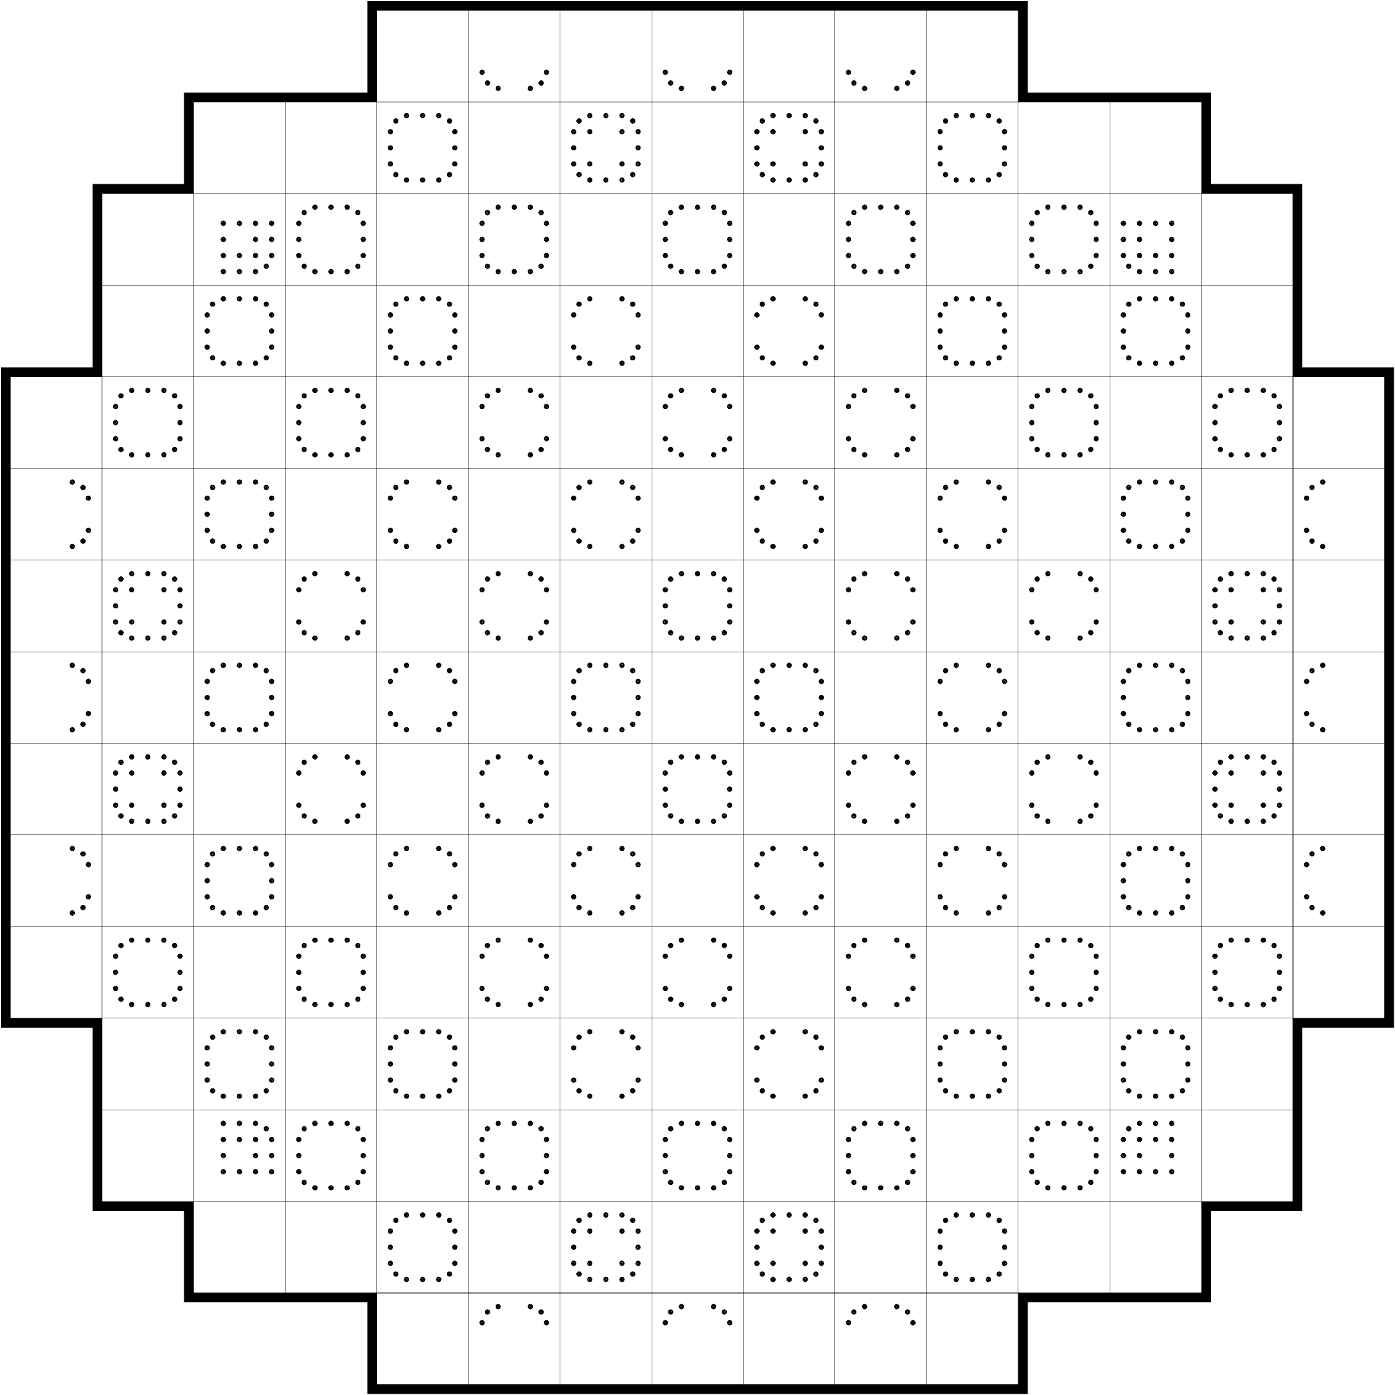
\includegraphics[width=6in]{specifications/core/figs/cat_ba_positions.png}
    \caption[Cycle 1 detailed burnable absorber view]{Detailed scale view of
    burnable absorber pins in cycle 1, showing proper rotations.
    \label{fig_ba_pos_real}}
\end{figure}

Figure \ref{fig_enr_ba_pos_c2} shows the shuffling pattern for cycle 2, which
includes 64 fresh assemblies and a different burnable absorber pattern.


\begin{figure}[htbp]
    \centering
    
    % these dimensions are determined in arrow_dimms.ods

    \def\scale{1.0}

    \def\latWidth{0.2673473684*\scale}
    
    \def\RPVOR{3*\scale}
    \def\rectW{0.75*\scale}
    \def\RPVIR{2.7315789474*\scale}
    \def\BarrelIR{2.3368421053*\scale}
    \def\BarrelOR{2.4078947368*\scale}
    \def\ShieldIR{2.4223787816*\scale}
    \def\ShieldOR{2.5067965189*\scale}
    \def\LinerIR{2.7246166598*\scale}

    \def\bafCIRx{0.9357157895*\scale}
    \def\bafCIRy{2.0051052632*\scale}
    \def\bafCORx{0.9633473684*\scale}
    \def\bafCORy{2.0327368421*\scale}
    \def\bafMIRx{1.7377578947*\scale}
    \def\bafMIRy{1.4704105263*\scale}
    \def\bafMORx{1.7653894737*\scale}
    \def\bafMORy{1.4980421053*\scale}
    
    \tikzset{Assembly/.style={
        inner sep=0pt,
        text width=\latWidth in,
        minimum size=\latWidth in,
        draw=black,
        align=center
        }
    }
    
    \def\tkzRPV{(0,0) circle (\RPVIR) (0,0) circle (\RPVOR)}
    \def\tkzLiner{(0,0) circle (\LinerIR) (0,0) circle (\RPVIR)}
    \def\tkzBarrel{(0,0) circle (\BarrelIR) (0,0) circle (\BarrelOR)}
    \def\tkzShields{(0,0) circle (\ShieldIR) (0,0) circle (\ShieldOR)}
    
    \def\tkzBaffCOR{(-\bafCORx, -\bafCORy) rectangle (\bafCORx, \bafCORy)}
    \def\tkzBaffCIR{(-\bafCIRx, -\bafCIRy) rectangle (\bafCIRx, \bafCIRy)} 
    \def\tkzBaffMOR{(-\bafMORx, -\bafMORy) rectangle (\bafMORx, \bafMORy)}
    \def\tkzBaffMIR{(-\bafMIRx, -\bafMIRy) rectangle (\bafMIRx, \bafMIRy) }
    \def\tkzBaffleC{ \tkzBaffCIR \tkzBaffCOR }
    \def\tkzBaffleM{ \tkzBaffMIR \tkzBaffMOR }

    \def\tkzBaffCClip{\tkzBaffCIR (-\RPVOR, -\RPVOR) rectangle (\RPVOR, \RPVOR)}
    \def\tkzBaffMClip{\tkzBaffMIR (-\RPVOR, -\RPVOR) rectangle (\RPVOR, \RPVOR)}

    \def\noenr{black!10}
    \def\lowenr{green!60!black}
    \def\highenr{orange!90}

    \scalebox{1.0}{

      \begin{tikzpicture}[x=1in,y=1in]
      
        % draw RPV, barrel, and shield panels
        
        \path[fill=black!90!white,even odd rule] \tkzRPV;
        \path[fill=black,even odd rule] \tkzLiner;
        \path[fill=black,even odd rule] \tkzBarrel;
        \begin{scope}
          \clip (0,0) -- +(61:\RPVOR) arc (61:29:\RPVOR) --
                (0,0) -- +(151:\RPVOR) arc (151:119:\RPVOR) -- 
                (0,0) -- +(241:\RPVOR) arc (241:209:\RPVOR) -- 
                (0,0) -- +(331:\RPVOR) arc (331:299:\RPVOR) -- cycle;
          \path[fill=black,even odd rule] \tkzShields;
        \end{scope}

        % draw baffle north/south
        
        \begin{scope}[even odd rule]
          \clip[rotate=90] \tkzBaffMClip;
          \path[fill=black] \tkzBaffleC;
        \end{scope}
        \begin{scope}[even odd rule]
          \clip \tkzBaffCClip;
          \clip \tkzBaffMClip;
          \path[fill=black, rotate=90] \tkzBaffleM;
        \end{scope}
        
        % draw baffle east/west
        
        \begin{scope}[rotate=90]
          \begin{scope}[even odd rule]
            \clip[rotate=90] \tkzBaffMClip;
            \path[fill=black] \tkzBaffleC;
          \end{scope}
          \begin{scope}[even odd rule]
            \clip \tkzBaffCClip;
            \clip \tkzBaffMClip;
            \path[fill=black, rotate=90] \tkzBaffleM;
          \end{scope}
        \end{scope}
        
        % draw assembly row/column headers
        
        \draw[red, thick] ($(-7*\latWidth,\RPVOR/\latWidth*\latWidth)$) node[above, anchor=south] {R} -- ($(-7*\latWidth,4*\latWidth)$);
        \draw[red, thick] ($(-6*\latWidth,\RPVOR/\latWidth*\latWidth)$) node[above, anchor=south] {P} -- ($(-6*\latWidth,6*\latWidth)$);
        \draw[red, thick] ($(-5*\latWidth,\RPVOR/\latWidth*\latWidth)$) node[above, anchor=south] {N} -- ($(-5*\latWidth,7*\latWidth)$);
        \draw[red, thick] ($(-4*\latWidth,\RPVOR/\latWidth*\latWidth)$) node[above, anchor=south] {M} -- ($(-4*\latWidth,7*\latWidth)$);
        \draw[red, thick] ($(-3*\latWidth,\RPVOR/\latWidth*\latWidth)$) node[above, anchor=south] {L} -- ($(-3*\latWidth,8*\latWidth)$);
        \draw[red, thick] ($(-2*\latWidth,\RPVOR/\latWidth*\latWidth)$) node[above, anchor=south] {K} -- ($(-2*\latWidth,8*\latWidth)$);
        \draw[red, thick] ($(-1*\latWidth,\RPVOR/\latWidth*\latWidth)$) node[above, anchor=south] {J} -- ($(-1*\latWidth,8*\latWidth)$);
        \draw[red, thick] ($(-0*\latWidth,\RPVOR/\latWidth*\latWidth)$) node[above, anchor=south] {H} -- ($(-0*\latWidth,8*\latWidth)$);
        \draw[red, thick] ($(1*\latWidth,\RPVOR/\latWidth*\latWidth)$) node[above, anchor=south] {G} -- ($(1*\latWidth,8*\latWidth)$);
        \draw[red, thick] ($(2*\latWidth,\RPVOR/\latWidth*\latWidth)$) node[above, anchor=south] {F} -- ($(2*\latWidth,8*\latWidth)$);
        \draw[red, thick] ($(3*\latWidth,\RPVOR/\latWidth*\latWidth)$) node[above, anchor=south] {E} -- ($(3*\latWidth,8*\latWidth)$);
        \draw[red, thick] ($(4*\latWidth,\RPVOR/\latWidth*\latWidth)$) node[above, anchor=south] {D} -- ($(4*\latWidth,7*\latWidth)$);
        \draw[red, thick] ($(5*\latWidth,\RPVOR/\latWidth*\latWidth)$) node[above, anchor=south] {C} -- ($(5*\latWidth,7*\latWidth)$);
        \draw[red, thick] ($(6*\latWidth,\RPVOR/\latWidth*\latWidth)$) node[above, anchor=south] {B} -- ($(6*\latWidth,6*\latWidth)$);
        \draw[red, thick] ($(7*\latWidth,\RPVOR/\latWidth*\latWidth)$) node[above, anchor=south] {A} -- ($(7*\latWidth,4*\latWidth)$);
        
        \begin{scope}[rotate=90]
          \draw[red, thick] ($(-7*\latWidth,\RPVOR/\latWidth*\latWidth)$) node[left, anchor=east] {15} -- ($(-7*\latWidth,4*\latWidth)$);
          \draw[red, thick] ($(-6*\latWidth,\RPVOR/\latWidth*\latWidth)$) node[left, anchor=east] {14} -- ($(-6*\latWidth,6*\latWidth)$);
          \draw[red, thick] ($(-5*\latWidth,\RPVOR/\latWidth*\latWidth)$) node[left, anchor=east] {13} -- ($(-5*\latWidth,7*\latWidth)$);
          \draw[red, thick] ($(-4*\latWidth,\RPVOR/\latWidth*\latWidth)$) node[left, anchor=east] {12} -- ($(-4*\latWidth,7*\latWidth)$);
          \draw[red, thick] ($(-3*\latWidth,\RPVOR/\latWidth*\latWidth)$) node[left, anchor=east] {11} -- ($(-3*\latWidth,8*\latWidth)$);
          \draw[red, thick] ($(-2*\latWidth,\RPVOR/\latWidth*\latWidth)$) node[left, anchor=east] {10} -- ($(-2*\latWidth,8*\latWidth)$);
          \draw[red, thick] ($(-1*\latWidth,\RPVOR/\latWidth*\latWidth)$) node[left, anchor=east] {9} -- ($(-1*\latWidth,8*\latWidth)$);
          \draw[red, thick] ($(-0*\latWidth,\RPVOR/\latWidth*\latWidth)$) node[left, anchor=east] {8} -- ($(-0*\latWidth,8*\latWidth)$);
          \draw[red, thick] ($(1*\latWidth,\RPVOR/\latWidth*\latWidth)$) node[left, anchor=east] {7} -- ($(1*\latWidth,8*\latWidth)$);
          \draw[red, thick] ($(2*\latWidth,\RPVOR/\latWidth*\latWidth)$) node[left, anchor=east] {6} -- ($(2*\latWidth,8*\latWidth)$);
          \draw[red, thick] ($(3*\latWidth,\RPVOR/\latWidth*\latWidth)$) node[left, anchor=east] {5} -- ($(3*\latWidth,8*\latWidth)$);
          \draw[red, thick] ($(4*\latWidth,\RPVOR/\latWidth*\latWidth)$) node[left, anchor=east] {4} -- ($(4*\latWidth,7*\latWidth)$);
          \draw[red, thick] ($(5*\latWidth,\RPVOR/\latWidth*\latWidth)$) node[left, anchor=east] {3} -- ($(5*\latWidth,7*\latWidth)$);
          \draw[red, thick] ($(6*\latWidth,\RPVOR/\latWidth*\latWidth)$) node[left, anchor=east] {2} -- ($(6*\latWidth,6*\latWidth)$);
          \draw[red, thick] ($(7*\latWidth,\RPVOR/\latWidth*\latWidth)$) node[left, anchor=east] {1} -- ($(7*\latWidth,4*\latWidth)$);
        \end{scope}
        
        % draw fuel assembly nodes
        
        \node [Assembly, fill=\noenr] at ($(-3*\latWidth,7*\latWidth)$) {\scriptsize L10}; % L1
        \node [Assembly, fill=\highenr] at ($(-2*\latWidth,7*\latWidth)$) {}; % K1
        \node [Assembly, fill=\lowenr] at ($(-1*\latWidth,7*\latWidth)$) {}; % J1
        \node [Assembly, fill=\highenr] at ($(-0*\latWidth,7*\latWidth)$) {}; % H1
        \node [Assembly, fill=\lowenr] at ($( 1*\latWidth,7*\latWidth)$) {}; % G1
        \node [Assembly, fill=\highenr] at ($( 2*\latWidth,7*\latWidth)$) {}; % F1
        \node [Assembly, fill=\noenr] at ($( 3*\latWidth,7*\latWidth)$) {\scriptsize E10}; % E1

        \node [Assembly, fill=\noenr] at ($(-5*\latWidth,6*\latWidth)$) {\scriptsize G10}; % N2
        \node [Assembly, fill=\lowenr] at ($(-4*\latWidth,6*\latWidth)$) {}; % M2
        \node [Assembly, fill=\lowenr, hyperlink node=ass_4ba_target] at ($(-3*\latWidth,6*\latWidth)$) {\small 4}; % L2
        \node [Assembly, fill=\noenr] at ($(-2*\latWidth,6*\latWidth)$) {\scriptsize L02}; % K2
        \node [Assembly, fill=\noenr] at ($(-1*\latWidth,6*\latWidth)$) {\scriptsize P12}; % J2
        \node [Assembly, fill=\noenr] at ($(-0*\latWidth,6*\latWidth)$) {\scriptsize N03}; % H2
        \node [Assembly, fill=\noenr] at ($( 1*\latWidth,6*\latWidth)$) {\scriptsize B12}; % G2
        \node [Assembly, fill=\noenr] at ($( 2*\latWidth,6*\latWidth)$) {\scriptsize E02}; % F2
        \node [Assembly, fill=\lowenr, hyperlink node=ass_4ba_target] at ($( 3*\latWidth,6*\latWidth)$) {\small 4}; % E2
        \node [Assembly, fill=\lowenr] at ($( 4*\latWidth,6*\latWidth)$) {}; % D2
        \node [Assembly, fill=\noenr] at ($( 5*\latWidth,6*\latWidth)$) {\scriptsize J10}; % C2

        \node [Assembly, fill=\noenr] at ($(-6*\latWidth,5*\latWidth)$) {\scriptsize F09}; % P3
        \node [Assembly, fill=\highenr] at ($(-5*\latWidth,5*\latWidth)$) {}; % N3
        \node [Assembly, fill=\noenr] at ($(-4*\latWidth,5*\latWidth)$) {\scriptsize N02}; % M3
        \node [Assembly, fill=\noenr] at ($(-3*\latWidth,5*\latWidth)$) {\scriptsize N10}; % L3
        \node [Assembly, fill=\lowenr, hyperlink node=ass_8ba_target] at ($(-2*\latWidth,5*\latWidth)$) {\small 8}; % K3
        \node [Assembly, fill=\noenr] at ($(-1*\latWidth,5*\latWidth)$) {\scriptsize D11}; % J3
        \node [Assembly, fill=\noenr] at ($(-0*\latWidth,5*\latWidth)$) {\scriptsize R10}; % H3
        \node [Assembly, fill=\noenr] at ($( 1*\latWidth,5*\latWidth)$) {\scriptsize M11}; % G3
        \node [Assembly, fill=\lowenr, hyperlink node=ass_8ba_target] at ($( 2*\latWidth,5*\latWidth)$) {\small 8}; % F3
        \node [Assembly, fill=\noenr] at ($( 3*\latWidth,5*\latWidth)$) {\scriptsize C10}; % E3
        \node [Assembly, fill=\noenr] at ($( 4*\latWidth,5*\latWidth)$) {\scriptsize C02}; % D3
        \node [Assembly, fill=\highenr] at ($( 5*\latWidth,5*\latWidth)$) {}; % C3
        \node [Assembly, fill=\noenr] at ($( 6*\latWidth,5*\latWidth)$) {\scriptsize K09}; % B3

        \node [Assembly, fill=\lowenr] at ($(-6*\latWidth,4*\latWidth)$) {}; % P4
        \node [Assembly, fill=\noenr] at ($(-5*\latWidth,4*\latWidth)$) {\scriptsize P03}; % N4
        \node [Assembly, fill=\noenr] at ($(-4*\latWidth,4*\latWidth)$) {\scriptsize L08}; % M4
        \node [Assembly, fill=\lowenr, hyperlink node=ass_12ba_c2_target] at ($(-3*\latWidth,4*\latWidth)$) {\small 12}; % L4
        \node [Assembly, fill=\noenr] at ($(-2*\latWidth,4*\latWidth)$) {\scriptsize M09}; % K4
        \node [Assembly, fill=\noenr] at ($(-1*\latWidth,4*\latWidth)$) {\scriptsize E15}; % J4
        \node [Assembly, fill=\noenr] at ($(-0*\latWidth,4*\latWidth)$) {\scriptsize G08}; % H4
        \node [Assembly, fill=\noenr] at ($( 1*\latWidth,4*\latWidth)$) {\scriptsize L15}; % G4
        \node [Assembly, fill=\noenr] at ($( 2*\latWidth,4*\latWidth)$) {\scriptsize D09}; % F4
        \node [Assembly, fill=\lowenr, hyperlink node=ass_12ba_c2_target] at ($( 3*\latWidth,4*\latWidth)$) {\small 12}; % E4
        \node [Assembly, fill=\noenr] at ($( 4*\latWidth,4*\latWidth)$) {\scriptsize H05}; % D4
        \node [Assembly, fill=\noenr] at ($( 5*\latWidth,4*\latWidth)$) {\scriptsize B03}; % C4
        \node [Assembly, fill=\lowenr] at ($( 6*\latWidth,4*\latWidth)$) {}; % B4

        \node [Assembly, fill=\noenr] at ($(-7*\latWidth,3*\latWidth)$) {\scriptsize F05}; % R5
        \node [Assembly, fill=\lowenr, hyperlink node=ass_4ba_target] at ($(-6*\latWidth,3*\latWidth)$) {\small 4}; % P5
        \node [Assembly, fill=\noenr] at ($(-5*\latWidth,3*\latWidth)$) {\scriptsize F03}; % N5
        \node [Assembly, fill=\lowenr, hyperlink node=ass_12ba_c2_target] at ($(-4*\latWidth,3*\latWidth)$) {\small 12}; % M5
        \node [Assembly, fill=\noenr] at ($(-3*\latWidth,3*\latWidth)$) {\scriptsize M04}; % L5
        \node [Assembly, fill=\lowenr, hyperlink node=ass_8ba_target] at ($(-2*\latWidth,3*\latWidth)$) {\small 8}; % K5
        \node [Assembly, fill=\noenr] at ($(-1*\latWidth,3*\latWidth)$) {\scriptsize M03}; % J5
        \node [Assembly, fill=\noenr] at ($(-0*\latWidth,3*\latWidth)$) {\scriptsize A10}; % H5
        \node [Assembly, fill=\noenr] at ($( 1*\latWidth,3*\latWidth)$) {\scriptsize D03}; % G5
        \node [Assembly, fill=\lowenr, hyperlink node=ass_8ba_target] at ($( 2*\latWidth,3*\latWidth)$) {\small 8}; % F5
        \node [Assembly, fill=\noenr] at ($( 3*\latWidth,3*\latWidth)$) {\scriptsize D04}; % E5
        \node [Assembly, fill=\lowenr, hyperlink node=ass_12ba_c2_target] at ($( 4*\latWidth,3*\latWidth)$) {\small 12}; % D5
        \node [Assembly, fill=\noenr] at ($( 5*\latWidth,3*\latWidth)$) {\scriptsize K03}; % C5
        \node [Assembly, fill=\lowenr, hyperlink node=ass_4ba_target] at ($( 6*\latWidth,3*\latWidth)$) {\small 4}; % B5
        \node [Assembly, fill=\noenr] at ($( 7*\latWidth,3*\latWidth)$) {\scriptsize K05}; % A5

        \node [Assembly, fill=\highenr] at ($(-7*\latWidth,2*\latWidth)$) {}; % R6
        \node [Assembly, fill=\noenr] at ($(-6*\latWidth,2*\latWidth)$) {\scriptsize P05}; % P6
        \node [Assembly, fill=\lowenr, hyperlink node=ass_8ba_target] at ($(-5*\latWidth,2*\latWidth)$) {\small 8}; % N6
        \node [Assembly, fill=\noenr] at ($(-4*\latWidth,2*\latWidth)$) {\scriptsize G04}; % M6
        \node [Assembly, fill=\lowenr, hyperlink node=ass_8ba_target] at ($(-3*\latWidth,2*\latWidth)$) {\small 8}; % L6
        \node [Assembly, fill=\noenr] at ($(-2*\latWidth,2*\latWidth)$) {\scriptsize N08}; % K6
        \node [Assembly, fill=\noenr] at ($(-1*\latWidth,2*\latWidth)$) {\scriptsize R09}; % J6
        \node [Assembly, fill=\noenr] at ($(-0*\latWidth,2*\latWidth)$) {\scriptsize G14}; % H6
        \node [Assembly, fill=\noenr] at ($( 1*\latWidth,2*\latWidth)$) {\scriptsize A09}; % G6
        \node [Assembly, fill=\noenr] at ($( 2*\latWidth,2*\latWidth)$) {\scriptsize H03}; % F6
        \node [Assembly, fill=\lowenr, hyperlink node=ass_8ba_target] at ($( 3*\latWidth,2*\latWidth)$) {\small 8}; % E6
        \node [Assembly, fill=\noenr] at ($( 4*\latWidth,2*\latWidth)$) {\scriptsize J04}; % D6
        \node [Assembly, fill=\lowenr, hyperlink node=ass_8ba_target] at ($( 5*\latWidth,2*\latWidth)$) {\small 8}; % C6
        \node [Assembly, fill=\noenr] at ($( 6*\latWidth,2*\latWidth)$) {\scriptsize B05}; % B6
        \node [Assembly, fill=\highenr] at ($( 7*\latWidth,2*\latWidth)$) {}; % A6

        \node [Assembly, fill=\lowenr] at ($(-7*\latWidth,1*\latWidth)$) {}; % R7
        \node [Assembly, fill=\noenr] at ($(-6*\latWidth,1*\latWidth)$) {\scriptsize D02}; % P7
        \node [Assembly, fill=\noenr] at ($(-5*\latWidth,1*\latWidth)$) {\scriptsize E12}; % N7
        \node [Assembly, fill=\noenr] at ($(-4*\latWidth,1*\latWidth)$) {\scriptsize A11}; % M7
        \node [Assembly, fill=\noenr] at ($(-3*\latWidth,1*\latWidth)$) {\scriptsize N04}; % L7
        \node [Assembly, fill=\noenr] at ($(-2*\latWidth,1*\latWidth)$) {\scriptsize G01}; % K7
        \node [Assembly, fill=\noenr] at ($(-1*\latWidth,1*\latWidth)$) {\scriptsize B09}; % J7
        \node [Assembly, fill=\noenr] at ($(-0*\latWidth,1*\latWidth)$) {\scriptsize H15}; % H7
        \node [Assembly, fill=\noenr] at ($( 1*\latWidth,1*\latWidth)$) {\scriptsize J14}; % G7
        \node [Assembly, fill=\noenr] at ($( 2*\latWidth,1*\latWidth)$) {\scriptsize J01}; % F7
        \node [Assembly, fill=\noenr] at ($( 3*\latWidth,1*\latWidth)$) {\scriptsize C04}; % E7
        \node [Assembly, fill=\noenr] at ($( 4*\latWidth,1*\latWidth)$) {\scriptsize R11}; % D7
        \node [Assembly, fill=\noenr] at ($( 5*\latWidth,1*\latWidth)$) {\scriptsize L12}; % C7
        \node [Assembly, fill=\noenr] at ($( 6*\latWidth,1*\latWidth)$) {\scriptsize M02}; % B7
        \node [Assembly, fill=\lowenr] at ($( 7*\latWidth,1*\latWidth)$) {}; % A7

        \node [Assembly, fill=\highenr] at ($(-7*\latWidth,0*\latWidth)$) {}; % R8
        \node [Assembly, fill=\noenr] at ($(-6*\latWidth,0*\latWidth)$) {\scriptsize N13}; % P8
        \node [Assembly, fill=\noenr] at ($(-5*\latWidth,0*\latWidth)$) {\scriptsize F15}; % N8
        \node [Assembly, fill=\noenr] at ($(-4*\latWidth,0*\latWidth)$) {\scriptsize H07}; % M8
        \node [Assembly, fill=\noenr] at ($(-3*\latWidth,0*\latWidth)$) {\scriptsize F01}; % L8
        \node [Assembly, fill=\noenr] at ($(-2*\latWidth,0*\latWidth)$) {\scriptsize B07}; % K8
        \node [Assembly, fill=\noenr] at ($(-1*\latWidth,0*\latWidth)$) {\scriptsize A08}; % J8
        \node [Assembly, fill=\noenr] at ($(-0*\latWidth,0*\latWidth)$) {\scriptsize F14}; % H8
        \node [Assembly, fill=\noenr] at ($( 1*\latWidth,0*\latWidth)$) {\scriptsize R08}; % G8
        \node [Assembly, fill=\noenr] at ($( 2*\latWidth,0*\latWidth)$) {\scriptsize P09}; % F8
        \node [Assembly, fill=\noenr] at ($( 3*\latWidth,0*\latWidth)$) {\scriptsize K15}; % E8
        \node [Assembly, fill=\noenr] at ($( 4*\latWidth,0*\latWidth)$) {\scriptsize H09}; % D8
        \node [Assembly, fill=\noenr] at ($( 5*\latWidth,0*\latWidth)$) {\scriptsize K01}; % C8
        \node [Assembly, fill=\noenr] at ($( 6*\latWidth,0*\latWidth)$) {\scriptsize C03}; % B8
        \node [Assembly, fill=\highenr] at ($( 7*\latWidth,0*\latWidth)$) {}; % A8

        \node [Assembly, fill=\lowenr] at ($(-7*\latWidth,-1*\latWidth)$) {}; % R9
        \node [Assembly, fill=\noenr] at ($(-6*\latWidth,-1*\latWidth)$) {\scriptsize D14}; % P9
        \node [Assembly, fill=\noenr] at ($(-5*\latWidth,-1*\latWidth)$) {\scriptsize E04}; % N9
        \node [Assembly, fill=\noenr] at ($(-4*\latWidth,-1*\latWidth)$) {\scriptsize A05}; % M9
        \node [Assembly, fill=\noenr] at ($(-3*\latWidth,-1*\latWidth)$) {\scriptsize N12}; % L9
        \node [Assembly, fill=\noenr] at ($(-2*\latWidth,-1*\latWidth)$) {\scriptsize G15}; % K9
        \node [Assembly, fill=\noenr] at ($(-1*\latWidth,-1*\latWidth)$) {\scriptsize G02}; % J9
        \node [Assembly, fill=\noenr] at ($(-0*\latWidth,-1*\latWidth)$) {\scriptsize H01}; % H9
        \node [Assembly, fill=\noenr] at ($( 1*\latWidth,-1*\latWidth)$) {\scriptsize P07}; % G9
        \node [Assembly, fill=\noenr] at ($( 2*\latWidth,-1*\latWidth)$) {\scriptsize J15}; % F9
        \node [Assembly, fill=\noenr] at ($( 3*\latWidth,-1*\latWidth)$) {\scriptsize C12}; % E9
        \node [Assembly, fill=\noenr] at ($( 4*\latWidth,-1*\latWidth)$) {\scriptsize R05}; % D9
        \node [Assembly, fill=\noenr] at ($( 5*\latWidth,-1*\latWidth)$) {\scriptsize L04}; % C9
        \node [Assembly, fill=\noenr] at ($( 6*\latWidth,-1*\latWidth)$) {\scriptsize M14}; % B9
        \node [Assembly, fill=\lowenr] at ($( 7*\latWidth,-1*\latWidth)$) {}; % A9

        \node [Assembly, fill=\highenr] at ($(-7*\latWidth,-2*\latWidth)$) {}; % R10
        \node [Assembly, fill=\noenr] at ($(-6*\latWidth,-2*\latWidth)$) {\scriptsize P11}; % P10
        \node [Assembly, fill=\lowenr, hyperlink node=ass_8ba_target] at ($(-5*\latWidth,-2*\latWidth)$) {\small 8}; % N10
        \node [Assembly, fill=\noenr] at ($(-4*\latWidth,-2*\latWidth)$) {\scriptsize G12}; % M10
        \node [Assembly, fill=\lowenr, hyperlink node=ass_8ba_target] at ($(-3*\latWidth,-2*\latWidth)$) {\small 8}; % L10
        \node [Assembly, fill=\noenr] at ($(-2*\latWidth,-2*\latWidth)$) {\scriptsize H13}; % K10
        \node [Assembly, fill=\noenr] at ($(-1*\latWidth,-2*\latWidth)$) {\scriptsize R07}; % J10
        \node [Assembly, fill=\noenr] at ($(-0*\latWidth,-2*\latWidth)$) {\scriptsize J02}; % H10
        \node [Assembly, fill=\noenr] at ($( 1*\latWidth,-2*\latWidth)$) {\scriptsize A07}; % G10
        \node [Assembly, fill=\noenr] at ($( 2*\latWidth,-2*\latWidth)$) {\scriptsize C08}; % F10
        \node [Assembly, fill=\lowenr, hyperlink node=ass_8ba_target] at ($( 3*\latWidth,-2*\latWidth)$) {\small 8}; % E10
        \node [Assembly, fill=\noenr] at ($( 4*\latWidth,-2*\latWidth)$) {\scriptsize J12}; % D10
        \node [Assembly, fill=\lowenr, hyperlink node=ass_8ba_target] at ($( 5*\latWidth,-2*\latWidth)$) {\small 8}; % C10
        \node [Assembly, fill=\noenr] at ($( 6*\latWidth,-2*\latWidth)$) {\scriptsize B11}; % B10
        \node [Assembly, fill=\highenr] at ($( 7*\latWidth,-2*\latWidth)$) {}; % A10

        \node [Assembly, fill=\noenr] at ($(-7*\latWidth,-3*\latWidth)$) {\scriptsize F11}; % R11
        \node [Assembly, fill=\lowenr, hyperlink node=ass_4ba_target] at ($(-6*\latWidth,-3*\latWidth)$) {\small 4}; % P11
        \node [Assembly, fill=\noenr] at ($(-5*\latWidth,-3*\latWidth)$) {\scriptsize F13}; % N11
        \node [Assembly, fill=\lowenr, hyperlink node=ass_12ba_c2_target] at ($(-4*\latWidth,-3*\latWidth)$) {\small 12}; % M11
        \node [Assembly, fill=\noenr] at ($(-3*\latWidth,-3*\latWidth)$) {\scriptsize M12}; % L11
        \node [Assembly, fill=\lowenr, hyperlink node=ass_8ba_target] at ($(-2*\latWidth,-3*\latWidth)$) {\small 8}; % K11
        \node [Assembly, fill=\noenr] at ($(-1*\latWidth,-3*\latWidth)$) {\scriptsize M13}; % J11
        \node [Assembly, fill=\noenr] at ($(-0*\latWidth,-3*\latWidth)$) {\scriptsize R06}; % H11
        \node [Assembly, fill=\noenr] at ($( 1*\latWidth,-3*\latWidth)$) {\scriptsize D13}; % G11
        \node [Assembly, fill=\lowenr, hyperlink node=ass_8ba_target] at ($( 2*\latWidth,-3*\latWidth)$) {\small 8}; % F11
        \node [Assembly, fill=\noenr] at ($( 3*\latWidth,-3*\latWidth)$) {\scriptsize D12}; % E11
        \node [Assembly, fill=\lowenr, hyperlink node=ass_12ba_c2_target] at ($( 4*\latWidth,-3*\latWidth)$) {\small 12}; % D11
        \node [Assembly, fill=\noenr] at ($( 5*\latWidth,-3*\latWidth)$) {\scriptsize K13}; % C11
        \node [Assembly, fill=\lowenr, hyperlink node=ass_4ba_target] at ($( 6*\latWidth,-3*\latWidth)$) {\small 4}; % B11
        \node [Assembly, fill=\noenr] at ($( 7*\latWidth,-3*\latWidth)$) {\scriptsize K11}; % A11

        \node [Assembly, fill=\lowenr] at ($(-6*\latWidth,-4*\latWidth)$) {}; % P12
        \node [Assembly, fill=\noenr] at ($(-5*\latWidth,-4*\latWidth)$) {\scriptsize P13}; % N12
        \node [Assembly, fill=\noenr] at ($(-4*\latWidth,-4*\latWidth)$) {\scriptsize H11}; % M12
        \node [Assembly, fill=\lowenr, hyperlink node=ass_12ba_c2_target] at ($(-3*\latWidth,-4*\latWidth)$) {\small 12}; % L12
        \node [Assembly, fill=\noenr] at ($(-2*\latWidth,-4*\latWidth)$) {\scriptsize M07}; % K12
        \node [Assembly, fill=\noenr] at ($(-1*\latWidth,-4*\latWidth)$) {\scriptsize E01}; % J12
        \node [Assembly, fill=\noenr] at ($(-0*\latWidth,-4*\latWidth)$) {\scriptsize J08}; % H12
        \node [Assembly, fill=\noenr] at ($( 1*\latWidth,-4*\latWidth)$) {\scriptsize L01}; % G12
        \node [Assembly, fill=\noenr] at ($( 2*\latWidth,-4*\latWidth)$) {\scriptsize D07}; % F12
        \node [Assembly, fill=\lowenr, hyperlink node=ass_12ba_c2_target] at ($( 3*\latWidth,-4*\latWidth)$) {\small 12}; % E12
        \node [Assembly, fill=\noenr] at ($( 4*\latWidth,-4*\latWidth)$) {\scriptsize E08}; % D12
        \node [Assembly, fill=\noenr] at ($( 5*\latWidth,-4*\latWidth)$) {\scriptsize B13}; % C12
        \node [Assembly, fill=\lowenr] at ($( 6*\latWidth,-4*\latWidth)$) {}; % B12

        \node [Assembly, fill=\noenr] at ($(-6*\latWidth,-5*\latWidth)$) {\scriptsize F07}; % P13
        \node [Assembly, fill=\highenr] at ($(-5*\latWidth,-5*\latWidth)$) {}; % N13
        \node [Assembly, fill=\noenr] at ($(-4*\latWidth,-5*\latWidth)$) {\scriptsize N14}; % M13
        \node [Assembly, fill=\noenr] at ($(-3*\latWidth,-5*\latWidth)$) {\scriptsize N06}; % L13
        \node [Assembly, fill=\lowenr, hyperlink node=ass_8ba_target] at ($(-2*\latWidth,-5*\latWidth)$) {\small 8}; % K13
        \node [Assembly, fill=\noenr] at ($(-1*\latWidth,-5*\latWidth)$) {\scriptsize D05}; % J13
        \node [Assembly, fill=\noenr] at ($(-0*\latWidth,-5*\latWidth)$) {\scriptsize A06}; % H13
        \node [Assembly, fill=\noenr] at ($( 1*\latWidth,-5*\latWidth)$) {\scriptsize M05}; % G13
        \node [Assembly, fill=\lowenr, hyperlink node=ass_8ba_target] at ($( 2*\latWidth,-5*\latWidth)$) {\small 8}; % F13
        \node [Assembly, fill=\noenr] at ($( 3*\latWidth,-5*\latWidth)$) {\scriptsize C06}; % E13
        \node [Assembly, fill=\noenr] at ($( 4*\latWidth,-5*\latWidth)$) {\scriptsize C14}; % D13
        \node [Assembly, fill=\highenr] at ($( 5*\latWidth,-5*\latWidth)$) {}; % C13
        \node [Assembly, fill=\noenr] at ($( 6*\latWidth,-5*\latWidth)$) {\scriptsize K07}; % B13

        \node [Assembly, fill=\noenr] at ($(-5*\latWidth,-6*\latWidth)$) {\scriptsize G06}; % N14
        \node [Assembly, fill=\lowenr] at ($(-4*\latWidth,-6*\latWidth)$) {}; % M14
        \node [Assembly, fill=\lowenr, hyperlink node=ass_4ba_target] at ($(-3*\latWidth,-6*\latWidth)$) {\small 4}; % L14
        \node [Assembly, fill=\noenr] at ($(-2*\latWidth,-6*\latWidth)$) {\scriptsize L14}; % K14
        \node [Assembly, fill=\noenr] at ($(-1*\latWidth,-6*\latWidth)$) {\scriptsize P04}; % J14
        \node [Assembly, fill=\noenr] at ($(-0*\latWidth,-6*\latWidth)$) {\scriptsize C13}; % H14
        \node [Assembly, fill=\noenr] at ($( 1*\latWidth,-6*\latWidth)$) {\scriptsize B04}; % G14
        \node [Assembly, fill=\noenr] at ($( 2*\latWidth,-6*\latWidth)$) {\scriptsize E14}; % F14
        \node [Assembly, fill=\lowenr, hyperlink node=ass_4ba_target] at ($( 3*\latWidth,-6*\latWidth)$) {\small 4}; % E14
        \node [Assembly, fill=\lowenr] at ($( 4*\latWidth,-6*\latWidth)$) {}; % D14
        \node [Assembly, fill=\noenr] at ($( 5*\latWidth,-6*\latWidth)$) {\scriptsize J06}; % C14

        \node [Assembly, fill=\noenr] at ($(-3*\latWidth,-7*\latWidth)$) {\scriptsize L06}; % L15
        \node [Assembly, fill=\highenr] at ($(-2*\latWidth,-7*\latWidth)$) {}; % K15
        \node [Assembly, fill=\lowenr] at ($(-1*\latWidth,-7*\latWidth)$) {}; % J15
        \node [Assembly, fill=\highenr] at ($(-0*\latWidth,-7*\latWidth)$) {}; % H15
        \node [Assembly, fill=\lowenr] at ($( 1*\latWidth,-7*\latWidth)$) {}; % G15
        \node [Assembly, fill=\highenr] at ($( 2*\latWidth,-7*\latWidth)$) {}; % F15
        \node [Assembly, fill=\noenr] at ($( 3*\latWidth,-7*\latWidth)$) {\scriptsize E06}; % E15
        
      \end{tikzpicture}
    }
    
    % make the legend
    \begin{tikzpicture}
      \matrix [matrix of nodes]
          {
              \node [Assembly, fill=\lowenr, hyperlink node=mat_fuel32] at (0,0) {}; & \hyperref[mat_fuel32]{Fresh 3.2 w/o U235}~~~ & \node [Assembly, fill=\highenr, hyperlink node=mat_fuel34] at (0,0) {}; & \hyperref[mat_fuel34]{Fresh 3.4 w/o U235}~~~ \\
              \node [Assembly, fill=\noenr] at (0,0) {}; & Shuffled Assembly~~~ & ~~~ & ~~~\\
          };
    \end{tikzpicture}

    \caption[Cycle 2 shuffling pattern and burnable absorber positions]{Cycle 2 shuffling pattern, burnable absorber positions, and enrichment loading pattern of fresh assemblies. Sources: \ref{num:assycore}, \ref{num:c2shuffle} \label{fig_enr_ba_pos_c2}}
\end{figure}

 % label: fig_enr_ba_pos_c2

%%%%%%%%%%%%%%%%%%%%%%%%%%%%%%%%%%%%%%%%%%%%%%%%%%%%%%%%%%%%%%%%%%%%%%%%%%%%%%%%
%\FloatBarrier
\paragraph{Control Rod Bank Positions}

Each of the four control rod banks - specified by the identifiers A, B, C, and D
- are made up of several control rod clusters in multiple fuel assemblies. In
control rod clusters, every guide tube is filled with the control rod pincell
described in section \ref{sec:pintypes}, with the exception of the center
tube. Each of the clusters in a given control rod bank move together.

In addition to the control rod banks, 5 shutdown banks of control rod clusters
are included above the core - specified by $\mathrm{S}_\mathrm{A}$,
$\mathrm{S}_\mathrm{B}$, $\mathrm{S}_\mathrm{C}$, $\mathrm{S}_\mathrm{D}$, and
$\mathrm{S}_\mathrm{E}$. These clusters are not used in normal operation,
however, their reactivity worth was measured and reported in Table
\ref{tbl:meas_c1phys}.

Figure \ref{fig_cr_pos} shows the radial locations of control rod clusters
belonging to each control rod and shutdown bank. The axial specifications of
each are described later in Section \ref{sec:axial_cr}.

The positions of control rod banks do not change between cycle 1 and cycle 2.


\begin{figure}[htbp]
    \centering
    
    % these dimensions are determined in arrow_dimms.ods

    \def\scale{1.0}

    \def\latWidth{0.2673473684*\scale}
    
    \def\RPVOR{3*\scale}
    \def\rectW{0.75*\scale}
    \def\RPVIR{2.7315789474*\scale}
    \def\BarrelIR{2.3368421053*\scale}
    \def\BarrelOR{2.4078947368*\scale}
    \def\ShieldIR{2.4223787816*\scale}
    \def\ShieldOR{2.5067965189*\scale}
    \def\LinerIR{2.7246166598*\scale}

    \def\bafCIRx{0.9357157895*\scale}
    \def\bafCIRy{2.0051052632*\scale}
    \def\bafCORx{0.9633473684*\scale}
    \def\bafCORy{2.0327368421*\scale}
    \def\bafMIRx{1.7377578947*\scale}
    \def\bafMIRy{1.4704105263*\scale}
    \def\bafMORx{1.7653894737*\scale}
    \def\bafMORy{1.4980421053*\scale}
    
    \tikzset{Assembly/.style={
        inner sep=0pt,
        text width=\latWidth in,
        minimum size=\latWidth in,
        draw=black,
        align=center
        }
    }
    
    \def\tkzRPV{(0,0) circle (\RPVIR) (0,0) circle (\RPVOR)}
    \def\tkzLiner{(0,0) circle (\LinerIR) (0,0) circle (\RPVIR)}
    \def\tkzBarrel{(0,0) circle (\BarrelIR) (0,0) circle (\BarrelOR)}
    \def\tkzShields{(0,0) circle (\ShieldIR) (0,0) circle (\ShieldOR)}
    
    \def\tkzBaffCOR{(-\bafCORx, -\bafCORy) rectangle (\bafCORx, \bafCORy)}
    \def\tkzBaffCIR{(-\bafCIRx, -\bafCIRy) rectangle (\bafCIRx, \bafCIRy)} 
    \def\tkzBaffMOR{(-\bafMORx, -\bafMORy) rectangle (\bafMORx, \bafMORy)}
    \def\tkzBaffMIR{(-\bafMIRx, -\bafMIRy) rectangle (\bafMIRx, \bafMIRy) }
    \def\tkzBaffleC{ \tkzBaffCIR \tkzBaffCOR }
    \def\tkzBaffleM{ \tkzBaffMIR \tkzBaffMOR }

    \def\tkzBaffCClip{\tkzBaffCIR (-\RPVOR, -\RPVOR) rectangle (\RPVOR, \RPVOR)}
    \def\tkzBaffMClip{\tkzBaffMIR (-\RPVOR, -\RPVOR) rectangle (\RPVOR, \RPVOR)}

    \def\highenr{blue!50}
    \def\midenr{yellow!50}
    \def\lowenr{red!50}

    \scalebox{1.0}{

      \begin{tikzpicture}[x=1in,y=1in]
      
        % draw RPV, barrel, liner and shield panels
        
        \path[fill=black!90!white,even odd rule] \tkzRPV;
        \path[fill=black,even odd rule] \tkzLiner;
        \path[fill=black,even odd rule] \tkzBarrel;
        \begin{scope}
          \clip (0,0) -- +(61:\RPVOR) arc (61:29:\RPVOR) --
                (0,0) -- +(151:\RPVOR) arc (151:119:\RPVOR) -- 
                (0,0) -- +(241:\RPVOR) arc (241:209:\RPVOR) -- 
                (0,0) -- +(331:\RPVOR) arc (331:299:\RPVOR) -- cycle;
          \path[fill=black,even odd rule] \tkzShields;
        \end{scope}

        % draw baffle north/south
        
        \begin{scope}[even odd rule]
          \clip[rotate=90] \tkzBaffMClip;
          \path[fill=black] \tkzBaffleC;
        \end{scope}
        \begin{scope}[even odd rule]
          \clip \tkzBaffCClip;
          \clip \tkzBaffMClip;
          \path[fill=black, rotate=90] \tkzBaffleM;
        \end{scope}
        
        % draw baffle east/west
        
        \begin{scope}[rotate=90]
          \begin{scope}[even odd rule]
            \clip[rotate=90] \tkzBaffMClip;
            \path[fill=black] \tkzBaffleC;
          \end{scope}
          \begin{scope}[even odd rule]
            \clip \tkzBaffCClip;
            \clip \tkzBaffMClip;
            \path[fill=black, rotate=90] \tkzBaffleM;
          \end{scope}
        \end{scope}
        
        % draw assembly row/column headers
        
        \draw[red, thick] ($(-7*\latWidth,\RPVOR/\latWidth*\latWidth)$) node[above, anchor=south] {R} -- ($(-7*\latWidth,4*\latWidth)$);
        \draw[red, thick] ($(-6*\latWidth,\RPVOR/\latWidth*\latWidth)$) node[above, anchor=south] {P} -- ($(-6*\latWidth,6*\latWidth)$);
        \draw[red, thick] ($(-5*\latWidth,\RPVOR/\latWidth*\latWidth)$) node[above, anchor=south] {N} -- ($(-5*\latWidth,7*\latWidth)$);
        \draw[red, thick] ($(-4*\latWidth,\RPVOR/\latWidth*\latWidth)$) node[above, anchor=south] {M} -- ($(-4*\latWidth,7*\latWidth)$);
        \draw[red, thick] ($(-3*\latWidth,\RPVOR/\latWidth*\latWidth)$) node[above, anchor=south] {L} -- ($(-3*\latWidth,8*\latWidth)$);
        \draw[red, thick] ($(-2*\latWidth,\RPVOR/\latWidth*\latWidth)$) node[above, anchor=south] {K} -- ($(-2*\latWidth,8*\latWidth)$);
        \draw[red, thick] ($(-1*\latWidth,\RPVOR/\latWidth*\latWidth)$) node[above, anchor=south] {J} -- ($(-1*\latWidth,8*\latWidth)$);
        \draw[red, thick] ($(-0*\latWidth,\RPVOR/\latWidth*\latWidth)$) node[above, anchor=south] {H} -- ($(-0*\latWidth,8*\latWidth)$);
        \draw[red, thick] ($(1*\latWidth,\RPVOR/\latWidth*\latWidth)$) node[above, anchor=south] {G} -- ($(1*\latWidth,8*\latWidth)$);
        \draw[red, thick] ($(2*\latWidth,\RPVOR/\latWidth*\latWidth)$) node[above, anchor=south] {F} -- ($(2*\latWidth,8*\latWidth)$);
        \draw[red, thick] ($(3*\latWidth,\RPVOR/\latWidth*\latWidth)$) node[above, anchor=south] {E} -- ($(3*\latWidth,8*\latWidth)$);
        \draw[red, thick] ($(4*\latWidth,\RPVOR/\latWidth*\latWidth)$) node[above, anchor=south] {D} -- ($(4*\latWidth,7*\latWidth)$);
        \draw[red, thick] ($(5*\latWidth,\RPVOR/\latWidth*\latWidth)$) node[above, anchor=south] {C} -- ($(5*\latWidth,7*\latWidth)$);
        \draw[red, thick] ($(6*\latWidth,\RPVOR/\latWidth*\latWidth)$) node[above, anchor=south] {B} -- ($(6*\latWidth,6*\latWidth)$);
        \draw[red, thick] ($(7*\latWidth,\RPVOR/\latWidth*\latWidth)$) node[above, anchor=south] {A} -- ($(7*\latWidth,4*\latWidth)$);
        
        \begin{scope}[rotate=90]
          \draw[red, thick] ($(-7*\latWidth,\RPVOR/\latWidth*\latWidth)$) node[left, anchor=east] {15} -- ($(-7*\latWidth,4*\latWidth)$);
          \draw[red, thick] ($(-6*\latWidth,\RPVOR/\latWidth*\latWidth)$) node[left, anchor=east] {14} -- ($(-6*\latWidth,6*\latWidth)$);
          \draw[red, thick] ($(-5*\latWidth,\RPVOR/\latWidth*\latWidth)$) node[left, anchor=east] {13} -- ($(-5*\latWidth,7*\latWidth)$);
          \draw[red, thick] ($(-4*\latWidth,\RPVOR/\latWidth*\latWidth)$) node[left, anchor=east] {12} -- ($(-4*\latWidth,7*\latWidth)$);
          \draw[red, thick] ($(-3*\latWidth,\RPVOR/\latWidth*\latWidth)$) node[left, anchor=east] {11} -- ($(-3*\latWidth,8*\latWidth)$);
          \draw[red, thick] ($(-2*\latWidth,\RPVOR/\latWidth*\latWidth)$) node[left, anchor=east] {10} -- ($(-2*\latWidth,8*\latWidth)$);
          \draw[red, thick] ($(-1*\latWidth,\RPVOR/\latWidth*\latWidth)$) node[left, anchor=east] {9} -- ($(-1*\latWidth,8*\latWidth)$);
          \draw[red, thick] ($(-0*\latWidth,\RPVOR/\latWidth*\latWidth)$) node[left, anchor=east] {8} -- ($(-0*\latWidth,8*\latWidth)$);
          \draw[red, thick] ($(1*\latWidth,\RPVOR/\latWidth*\latWidth)$) node[left, anchor=east] {7} -- ($(1*\latWidth,8*\latWidth)$);
          \draw[red, thick] ($(2*\latWidth,\RPVOR/\latWidth*\latWidth)$) node[left, anchor=east] {6} -- ($(2*\latWidth,8*\latWidth)$);
          \draw[red, thick] ($(3*\latWidth,\RPVOR/\latWidth*\latWidth)$) node[left, anchor=east] {5} -- ($(3*\latWidth,8*\latWidth)$);
          \draw[red, thick] ($(4*\latWidth,\RPVOR/\latWidth*\latWidth)$) node[left, anchor=east] {4} -- ($(4*\latWidth,7*\latWidth)$);
          \draw[red, thick] ($(5*\latWidth,\RPVOR/\latWidth*\latWidth)$) node[left, anchor=east] {3} -- ($(5*\latWidth,7*\latWidth)$);
          \draw[red, thick] ($(6*\latWidth,\RPVOR/\latWidth*\latWidth)$) node[left, anchor=east] {2} -- ($(6*\latWidth,6*\latWidth)$);
          \draw[red, thick] ($(7*\latWidth,\RPVOR/\latWidth*\latWidth)$) node[left, anchor=east] {1} -- ($(7*\latWidth,4*\latWidth)$);
        \end{scope}
        
        % draw fuel assembly nodes
        
        \node [Assembly, fill=\highenr] at ($(-3*\latWidth,7*\latWidth)$) {}; % L1
        \node [Assembly, fill=\highenr] at ($(-2*\latWidth,7*\latWidth)$) {}; % K1
        \node [Assembly, fill=\highenr] at ($(-1*\latWidth,7*\latWidth)$) {}; % J1
        \node [Assembly, fill=\highenr] at ($(-0*\latWidth,7*\latWidth)$) {}; % H1
        \node [Assembly, fill=\highenr] at ($( 1*\latWidth,7*\latWidth)$) {}; % G1
        \node [Assembly, fill=\highenr] at ($( 2*\latWidth,7*\latWidth)$) {}; % F1
        \node [Assembly, fill=\highenr] at ($( 3*\latWidth,7*\latWidth)$) {}; % E1

        \node [Assembly, fill=\highenr] at ($(-5*\latWidth,6*\latWidth)$) {}; % N2
        \node [Assembly, fill=\highenr] at ($(-4*\latWidth,6*\latWidth)$) {$\mathrm{S}_\mathrm{A}$}; % M2
        \node [Assembly, fill=\highenr] at ($(-3*\latWidth,6*\latWidth)$) {}; % L2
        \node [Assembly, fill=\lowenr] at ($(-2*\latWidth,6*\latWidth)$) {$\mathrm{B}$}; % K2
        \node [Assembly, fill=\highenr] at ($(-1*\latWidth,6*\latWidth)$) {}; % J2
        \node [Assembly, fill=\lowenr] at ($(-0*\latWidth,6*\latWidth)$) {$\mathrm{C}$}; % H2
        \node [Assembly, fill=\highenr] at ($( 1*\latWidth,6*\latWidth)$) {}; % G2
        \node [Assembly, fill=\lowenr] at ($( 2*\latWidth,6*\latWidth)$) {$\mathrm{B}$}; % F2
        \node [Assembly, fill=\highenr] at ($( 3*\latWidth,6*\latWidth)$) {}; % E2
        \node [Assembly, fill=\highenr] at ($( 4*\latWidth,6*\latWidth)$) {$\mathrm{S}_\mathrm{A}$}; % D2
        \node [Assembly, fill=\highenr] at ($( 5*\latWidth,6*\latWidth)$) {}; % C2

        \node [Assembly, fill=\highenr] at ($(-6*\latWidth,5*\latWidth)$) {}; % P3
        \node [Assembly, fill=\highenr] at ($(-5*\latWidth,5*\latWidth)$) {}; % N3
        \node [Assembly, fill=\midenr] at ($(-4*\latWidth,5*\latWidth)$) {}; % M3
        \node [Assembly, fill=\lowenr] at ($(-3*\latWidth,5*\latWidth)$) {$\mathrm{S}_\mathrm{D}$}; % L3
        \node [Assembly, fill=\midenr] at ($(-2*\latWidth,5*\latWidth)$) {}; % K3
        \node [Assembly, fill=\lowenr] at ($(-1*\latWidth,5*\latWidth)$) {$\mathrm{S}_\mathrm{B}$}; % J3
        \node [Assembly, fill=\midenr] at ($(-0*\latWidth,5*\latWidth)$) {}; % H3
        \node [Assembly, fill=\lowenr] at ($( 1*\latWidth,5*\latWidth)$) {$\mathrm{S}_\mathrm{B}$}; % G3
        \node [Assembly, fill=\midenr] at ($( 2*\latWidth,5*\latWidth)$) {}; % F3
        \node [Assembly, fill=\lowenr] at ($( 3*\latWidth,5*\latWidth)$) {$\mathrm{S}_\mathrm{C}$}; % E3
        \node [Assembly, fill=\midenr] at ($( 4*\latWidth,5*\latWidth)$) {}; % D3
        \node [Assembly, fill=\highenr] at ($( 5*\latWidth,5*\latWidth)$) {}; % C3
        \node [Assembly, fill=\highenr] at ($( 6*\latWidth,5*\latWidth)$) {}; % B3

        \node [Assembly, fill=\highenr] at ($(-6*\latWidth,4*\latWidth)$) {$\mathrm{S}_\mathrm{A}$}; % P4
        \node [Assembly, fill=\midenr] at ($(-5*\latWidth,4*\latWidth)$) {}; % N4
        \node [Assembly, fill=\midenr] at ($(-4*\latWidth,4*\latWidth)$) {$\mathrm{D}$}; % M4
        \node [Assembly, fill=\midenr] at ($(-3*\latWidth,4*\latWidth)$) {}; % L4
        \node [Assembly, fill=\lowenr] at ($(-2*\latWidth,4*\latWidth)$) {}; % K4
        \node [Assembly, fill=\midenr] at ($(-1*\latWidth,4*\latWidth)$) {}; % J4
        \node [Assembly, fill=\lowenr] at ($(-0*\latWidth,4*\latWidth)$) {$\mathrm{S}_\mathrm{E}$}; % H4
        \node [Assembly, fill=\midenr] at ($( 1*\latWidth,4*\latWidth)$) {}; % G4
        \node [Assembly, fill=\lowenr] at ($( 2*\latWidth,4*\latWidth)$) {}; % F4
        \node [Assembly, fill=\midenr] at ($( 3*\latWidth,4*\latWidth)$) {}; % E4
        \node [Assembly, fill=\midenr] at ($( 4*\latWidth,4*\latWidth)$) {$\mathrm{D}$}; % D4
        \node [Assembly, fill=\midenr] at ($( 5*\latWidth,4*\latWidth)$) {}; % C4
        \node [Assembly, fill=\highenr] at ($( 6*\latWidth,4*\latWidth)$) {$\mathrm{S}_\mathrm{A}$}; % B4

        \node [Assembly, fill=\highenr] at ($(-7*\latWidth,3*\latWidth)$) {}; % R5
        \node [Assembly, fill=\highenr] at ($(-6*\latWidth,3*\latWidth)$) {}; % P5
        \node [Assembly, fill=\lowenr] at ($(-5*\latWidth,3*\latWidth)$) {$\mathrm{S}_\mathrm{C}$}; % N5
        \node [Assembly, fill=\midenr] at ($(-4*\latWidth,3*\latWidth)$) {}; % M5
        \node [Assembly, fill=\lowenr] at ($(-3*\latWidth,3*\latWidth)$) {}; % L5
        \node [Assembly, fill=\midenr] at ($(-2*\latWidth,3*\latWidth)$) {}; % K5
        \node [Assembly, fill=\lowenr] at ($(-1*\latWidth,3*\latWidth)$) {}; % J5
        \node [Assembly, fill=\midenr] at ($(-0*\latWidth,3*\latWidth)$) {}; % H5
        \node [Assembly, fill=\lowenr] at ($( 1*\latWidth,3*\latWidth)$) {}; % G5
        \node [Assembly, fill=\midenr] at ($( 2*\latWidth,3*\latWidth)$) {}; % F5
        \node [Assembly, fill=\lowenr] at ($( 3*\latWidth,3*\latWidth)$) {}; % E5
        \node [Assembly, fill=\midenr] at ($( 4*\latWidth,3*\latWidth)$) {}; % D5
        \node [Assembly, fill=\lowenr] at ($( 5*\latWidth,3*\latWidth)$) {$\mathrm{S}_\mathrm{D}$}; % C5
        \node [Assembly, fill=\highenr] at ($( 6*\latWidth,3*\latWidth)$) {}; % B5
        \node [Assembly, fill=\highenr] at ($( 7*\latWidth,3*\latWidth)$) {}; % A5

        \node [Assembly, fill=\highenr] at ($(-7*\latWidth,2*\latWidth)$) {}; % R6
        \node [Assembly, fill=\lowenr] at ($(-6*\latWidth,2*\latWidth)$) {$\mathrm{B}$}; % P6
        \node [Assembly, fill=\midenr] at ($(-5*\latWidth,2*\latWidth)$) {}; % N6
        \node [Assembly, fill=\lowenr] at ($(-4*\latWidth,2*\latWidth)$) {}; % M6
        \node [Assembly, fill=\midenr] at ($(-3*\latWidth,2*\latWidth)$) {}; % L6
        \node [Assembly, fill=\lowenr] at ($(-2*\latWidth,2*\latWidth)$) {$\mathrm{C}$}; % K6
        \node [Assembly, fill=\midenr] at ($(-1*\latWidth,2*\latWidth)$) {}; % J6
        \node [Assembly, fill=\lowenr] at ($(-0*\latWidth,2*\latWidth)$) {$\mathrm{A}$}; % H6
        \node [Assembly, fill=\midenr] at ($( 1*\latWidth,2*\latWidth)$) {}; % G6
        \node [Assembly, fill=\lowenr] at ($( 2*\latWidth,2*\latWidth)$) {$\mathrm{C}$}; % F6
        \node [Assembly, fill=\midenr] at ($( 3*\latWidth,2*\latWidth)$) {}; % E6
        \node [Assembly, fill=\lowenr] at ($( 4*\latWidth,2*\latWidth)$) {}; % D6
        \node [Assembly, fill=\midenr] at ($( 5*\latWidth,2*\latWidth)$) {}; % C6
        \node [Assembly, fill=\lowenr] at ($( 6*\latWidth,2*\latWidth)$) {$\mathrm{B}$}; % B6
        \node [Assembly, fill=\highenr] at ($( 7*\latWidth,2*\latWidth)$) {}; % A6

        \node [Assembly, fill=\highenr] at ($(-7*\latWidth,1*\latWidth)$) {}; % R7
        \node [Assembly, fill=\highenr] at ($(-6*\latWidth,1*\latWidth)$) {}; % P7
        \node [Assembly, fill=\lowenr] at ($(-5*\latWidth,1*\latWidth)$) {$\mathrm{S}_\mathrm{B}$}; % N7
        \node [Assembly, fill=\midenr] at ($(-4*\latWidth,1*\latWidth)$) {}; % M7
        \node [Assembly, fill=\lowenr] at ($(-3*\latWidth,1*\latWidth)$) {}; % L7
        \node [Assembly, fill=\midenr] at ($(-2*\latWidth,1*\latWidth)$) {}; % K7
        \node [Assembly, fill=\lowenr] at ($(-1*\latWidth,1*\latWidth)$) {}; % J7
        \node [Assembly, fill=\midenr] at ($(-0*\latWidth,1*\latWidth)$) {}; % H7
        \node [Assembly, fill=\lowenr] at ($( 1*\latWidth,1*\latWidth)$) {}; % G7
        \node [Assembly, fill=\midenr] at ($( 2*\latWidth,1*\latWidth)$) {}; % F7
        \node [Assembly, fill=\lowenr] at ($( 3*\latWidth,1*\latWidth)$) {}; % E7
        \node [Assembly, fill=\midenr] at ($( 4*\latWidth,1*\latWidth)$) {}; % D7
        \node [Assembly, fill=\lowenr] at ($( 5*\latWidth,1*\latWidth)$) {$\mathrm{S}_\mathrm{B}$}; % C7
        \node [Assembly, fill=\highenr] at ($( 6*\latWidth,1*\latWidth)$) {}; % B7
        \node [Assembly, fill=\highenr] at ($( 7*\latWidth,1*\latWidth)$) {}; % A7

        \node [Assembly, fill=\highenr] at ($(-7*\latWidth,0*\latWidth)$) {}; % R8
        \node [Assembly, fill=\lowenr] at ($(-6*\latWidth,0*\latWidth)$) {$\mathrm{C}$}; % P8
        \node [Assembly, fill=\midenr] at ($(-5*\latWidth,0*\latWidth)$) {}; % N8
        \node [Assembly, fill=\lowenr] at ($(-4*\latWidth,0*\latWidth)$) {$\mathrm{S}_\mathrm{E}$}; % M8
        \node [Assembly, fill=\midenr] at ($(-3*\latWidth,0*\latWidth)$) {}; % L8
        \node [Assembly, fill=\lowenr] at ($(-2*\latWidth,0*\latWidth)$) {$\mathrm{A}$}; % K8
        \node [Assembly, fill=\midenr] at ($(-1*\latWidth,0*\latWidth)$) {}; % J8
        \node [Assembly, fill=\lowenr] at ($(-0*\latWidth,0*\latWidth)$) {$\mathrm{D}$}; % H8
        \node [Assembly, fill=\midenr] at ($( 1*\latWidth,0*\latWidth)$) {}; % G8
        \node [Assembly, fill=\lowenr] at ($( 2*\latWidth,0*\latWidth)$) {$\mathrm{A}$}; % F8
        \node [Assembly, fill=\midenr] at ($( 3*\latWidth,0*\latWidth)$) {}; % E8
        \node [Assembly, fill=\lowenr] at ($( 4*\latWidth,0*\latWidth)$) {$\mathrm{S}_\mathrm{E}$}; % D8
        \node [Assembly, fill=\midenr] at ($( 5*\latWidth,0*\latWidth)$) {}; % C8
        \node [Assembly, fill=\lowenr] at ($( 6*\latWidth,0*\latWidth)$) {$\mathrm{C}$}; % B8
        \node [Assembly, fill=\highenr] at ($( 7*\latWidth,0*\latWidth)$) {}; % A8

        \node [Assembly, fill=\highenr] at ($(-7*\latWidth,-1*\latWidth)$) {}; % R9
        \node [Assembly, fill=\highenr] at ($(-6*\latWidth,-1*\latWidth)$) {}; % P9
        \node [Assembly, fill=\lowenr] at ($(-5*\latWidth,-1*\latWidth)$) {$\mathrm{S}_\mathrm{B}$}; % N9
        \node [Assembly, fill=\midenr] at ($(-4*\latWidth,-1*\latWidth)$) {}; % M9
        \node [Assembly, fill=\lowenr] at ($(-3*\latWidth,-1*\latWidth)$) {}; % L9
        \node [Assembly, fill=\midenr] at ($(-2*\latWidth,-1*\latWidth)$) {}; % K9
        \node [Assembly, fill=\lowenr] at ($(-1*\latWidth,-1*\latWidth)$) {}; % J9
        \node [Assembly, fill=\midenr] at ($(-0*\latWidth,-1*\latWidth)$) {}; % H9
        \node [Assembly, fill=\lowenr] at ($( 1*\latWidth,-1*\latWidth)$) {}; % G9
        \node [Assembly, fill=\midenr] at ($( 2*\latWidth,-1*\latWidth)$) {}; % F9
        \node [Assembly, fill=\lowenr] at ($( 3*\latWidth,-1*\latWidth)$) {}; % E9
        \node [Assembly, fill=\midenr] at ($( 4*\latWidth,-1*\latWidth)$) {}; % D9
        \node [Assembly, fill=\lowenr] at ($( 5*\latWidth,-1*\latWidth)$) {$\mathrm{S}_\mathrm{B}$}; % C9
        \node [Assembly, fill=\highenr] at ($( 6*\latWidth,-1*\latWidth)$) {}; % B9
        \node [Assembly, fill=\highenr] at ($( 7*\latWidth,-1*\latWidth)$) {}; % A9

        \node [Assembly, fill=\highenr] at ($(-7*\latWidth,-2*\latWidth)$) {}; % R10
        \node [Assembly, fill=\lowenr] at ($(-6*\latWidth,-2*\latWidth)$) {$\mathrm{B}$}; % P10
        \node [Assembly, fill=\midenr] at ($(-5*\latWidth,-2*\latWidth)$) {}; % N10
        \node [Assembly, fill=\lowenr] at ($(-4*\latWidth,-2*\latWidth)$) {}; % M10
        \node [Assembly, fill=\midenr] at ($(-3*\latWidth,-2*\latWidth)$) {}; % L10
        \node [Assembly, fill=\lowenr] at ($(-2*\latWidth,-2*\latWidth)$) {$\mathrm{C}$}; % K10
        \node [Assembly, fill=\midenr] at ($(-1*\latWidth,-2*\latWidth)$) {}; % J10
        \node [Assembly, fill=\lowenr] at ($(-0*\latWidth,-2*\latWidth)$) {$\mathrm{A}$}; % H10
        \node [Assembly, fill=\midenr] at ($( 1*\latWidth,-2*\latWidth)$) {}; % G10
        \node [Assembly, fill=\lowenr] at ($( 2*\latWidth,-2*\latWidth)$) {$\mathrm{C}$}; % F10
        \node [Assembly, fill=\midenr] at ($( 3*\latWidth,-2*\latWidth)$) {}; % E10
        \node [Assembly, fill=\lowenr] at ($( 4*\latWidth,-2*\latWidth)$) {}; % D10
        \node [Assembly, fill=\midenr] at ($( 5*\latWidth,-2*\latWidth)$) {}; % C10
        \node [Assembly, fill=\lowenr] at ($( 6*\latWidth,-2*\latWidth)$) {$\mathrm{B}$}; % B10
        \node [Assembly, fill=\highenr] at ($( 7*\latWidth,-2*\latWidth)$) {}; % A10

        \node [Assembly, fill=\highenr] at ($(-7*\latWidth,-3*\latWidth)$) {}; % R11
        \node [Assembly, fill=\highenr] at ($(-6*\latWidth,-3*\latWidth)$) {}; % P11
        \node [Assembly, fill=\lowenr] at ($(-5*\latWidth,-3*\latWidth)$) {$\mathrm{S}_\mathrm{D}$}; % N11
        \node [Assembly, fill=\midenr] at ($(-4*\latWidth,-3*\latWidth)$) {}; % M11
        \node [Assembly, fill=\lowenr] at ($(-3*\latWidth,-3*\latWidth)$) {}; % L11
        \node [Assembly, fill=\midenr] at ($(-2*\latWidth,-3*\latWidth)$) {}; % K11
        \node [Assembly, fill=\lowenr] at ($(-1*\latWidth,-3*\latWidth)$) {}; % J11
        \node [Assembly, fill=\midenr] at ($(-0*\latWidth,-3*\latWidth)$) {}; % H11
        \node [Assembly, fill=\lowenr] at ($( 1*\latWidth,-3*\latWidth)$) {}; % G11
        \node [Assembly, fill=\midenr] at ($( 2*\latWidth,-3*\latWidth)$) {}; % F11
        \node [Assembly, fill=\lowenr] at ($( 3*\latWidth,-3*\latWidth)$) {}; % E11
        \node [Assembly, fill=\midenr] at ($( 4*\latWidth,-3*\latWidth)$) {}; % D11
        \node [Assembly, fill=\lowenr] at ($( 5*\latWidth,-3*\latWidth)$) {$\mathrm{S}_\mathrm{C}$}; % C11
        \node [Assembly, fill=\highenr] at ($( 6*\latWidth,-3*\latWidth)$) {}; % B11
        \node [Assembly, fill=\highenr] at ($( 7*\latWidth,-3*\latWidth)$) {}; % A11

        \node [Assembly, fill=\highenr] at ($(-6*\latWidth,-4*\latWidth)$) {$\mathrm{S}_\mathrm{A}$}; % P12
        \node [Assembly, fill=\midenr] at ($(-5*\latWidth,-4*\latWidth)$) {}; % N12
        \node [Assembly, fill=\midenr] at ($(-4*\latWidth,-4*\latWidth)$) {$\mathrm{D}$}; % M12
        \node [Assembly, fill=\midenr] at ($(-3*\latWidth,-4*\latWidth)$) {}; % L12
        \node [Assembly, fill=\lowenr] at ($(-2*\latWidth,-4*\latWidth)$) {}; % K12
        \node [Assembly, fill=\midenr] at ($(-1*\latWidth,-4*\latWidth)$) {}; % J12
        \node [Assembly, fill=\lowenr] at ($(-0*\latWidth,-4*\latWidth)$) {$\mathrm{S}_\mathrm{E}$}; % H12
        \node [Assembly, fill=\midenr] at ($( 1*\latWidth,-4*\latWidth)$) {}; % G12
        \node [Assembly, fill=\lowenr] at ($( 2*\latWidth,-4*\latWidth)$) {}; % F12
        \node [Assembly, fill=\midenr] at ($( 3*\latWidth,-4*\latWidth)$) {}; % E12
        \node [Assembly, fill=\midenr] at ($( 4*\latWidth,-4*\latWidth)$) {$\mathrm{D}$}; % D12
        \node [Assembly, fill=\midenr] at ($( 5*\latWidth,-4*\latWidth)$) {}; % C12
        \node [Assembly, fill=\highenr] at ($( 6*\latWidth,-4*\latWidth)$) {$\mathrm{S}_\mathrm{A}$}; % B12

        \node [Assembly, fill=\highenr] at ($(-6*\latWidth,-5*\latWidth)$) {}; % P13
        \node [Assembly, fill=\highenr] at ($(-5*\latWidth,-5*\latWidth)$) {}; % N13
        \node [Assembly, fill=\midenr] at ($(-4*\latWidth,-5*\latWidth)$) {}; % M13
        \node [Assembly, fill=\lowenr] at ($(-3*\latWidth,-5*\latWidth)$) {$\mathrm{S}_\mathrm{C}$}; % L13
        \node [Assembly, fill=\midenr] at ($(-2*\latWidth,-5*\latWidth)$) {}; % K13
        \node [Assembly, fill=\lowenr] at ($(-1*\latWidth,-5*\latWidth)$) {$\mathrm{S}_\mathrm{B}$}; % J13
        \node [Assembly, fill=\midenr] at ($(-0*\latWidth,-5*\latWidth)$) {}; % H13
        \node [Assembly, fill=\lowenr] at ($( 1*\latWidth,-5*\latWidth)$) {$\mathrm{S}_\mathrm{B}$}; % G13
        \node [Assembly, fill=\midenr] at ($( 2*\latWidth,-5*\latWidth)$) {}; % F13
        \node [Assembly, fill=\lowenr] at ($( 3*\latWidth,-5*\latWidth)$) {$\mathrm{S}_\mathrm{D}$}; % E13
        \node [Assembly, fill=\midenr] at ($( 4*\latWidth,-5*\latWidth)$) {}; % D13
        \node [Assembly, fill=\highenr] at ($( 5*\latWidth,-5*\latWidth)$) {}; % C13
        \node [Assembly, fill=\highenr] at ($( 6*\latWidth,-5*\latWidth)$) {}; % B13

        \node [Assembly, fill=\highenr] at ($(-5*\latWidth,-6*\latWidth)$) {}; % N14
        \node [Assembly, fill=\highenr] at ($(-4*\latWidth,-6*\latWidth)$) {$\mathrm{S}_\mathrm{A}$}; % M14
        \node [Assembly, fill=\highenr] at ($(-3*\latWidth,-6*\latWidth)$) {}; % L14
        \node [Assembly, fill=\lowenr] at ($(-2*\latWidth,-6*\latWidth)$) {$\mathrm{B}$}; % K14
        \node [Assembly, fill=\highenr] at ($(-1*\latWidth,-6*\latWidth)$) {}; % J14
        \node [Assembly, fill=\lowenr] at ($(-0*\latWidth,-6*\latWidth)$) {$\mathrm{C}$}; % H14
        \node [Assembly, fill=\highenr] at ($( 1*\latWidth,-6*\latWidth)$) {}; % G14
        \node [Assembly, fill=\lowenr] at ($( 2*\latWidth,-6*\latWidth)$) {$\mathrm{B}$}; % F14
        \node [Assembly, fill=\highenr] at ($( 3*\latWidth,-6*\latWidth)$) {}; % E14
        \node [Assembly, fill=\highenr] at ($( 4*\latWidth,-6*\latWidth)$) {$\mathrm{S}_\mathrm{A}$}; % D14
        \node [Assembly, fill=\highenr] at ($( 5*\latWidth,-6*\latWidth)$) {}; % C14

        \node [Assembly, fill=\highenr] at ($(-3*\latWidth,-7*\latWidth)$) {}; % L15
        \node [Assembly, fill=\highenr] at ($(-2*\latWidth,-7*\latWidth)$) {}; % K15
        \node [Assembly, fill=\highenr] at ($(-1*\latWidth,-7*\latWidth)$) {}; % J15
        \node [Assembly, fill=\highenr] at ($(-0*\latWidth,-7*\latWidth)$) {}; % H15
        \node [Assembly, fill=\highenr] at ($( 1*\latWidth,-7*\latWidth)$) {}; % G15
        \node [Assembly, fill=\highenr] at ($( 2*\latWidth,-7*\latWidth)$) {}; % F15
        \node [Assembly, fill=\highenr] at ($( 3*\latWidth,-7*\latWidth)$) {}; % E15

      \end{tikzpicture}
    }
    


    \caption[Control rod and shutdown bank positions.]{Control rod and shutdown bank positions. Source: \ref{num:assycore} \label{fig_cr_pos}}
\end{figure}

 % label: fig_cr_pos

%%%%%%%%%%%%%%%%%%%%%%%%%%%%%%%%%%%%%%%%%%%%%%%%%%%%%%%%%%%%%%%%%%%%%%%%%%%%%%%%
\FloatBarrier
\paragraph{Instrument Tube Positions}
\label{sec:coreinstrpos}

The central guide tube for many fuel assemblies in the core is filled by an
instrument tube, as described in Section \ref{sec:pintypes}. Figure
\ref{fig_instr_pos} shows these positions. Where not indicated, the central
guide tube is filled with water, as described in section \ref{sec:pintypes}.

The positions of instrument tubes do not change between cycle 1 and cycle 2.


\begin{figure}[htbp]
    \centering
    
    % these dimensions are determined in arrow_dimms.ods

    \def\scale{1.0}

    \def\latWidth{0.2673473684*\scale}
    
    \def\RPVOR{3*\scale}
    \def\rectW{0.75*\scale}
    \def\RPVIR{2.7315789474*\scale}
    \def\BarrelIR{2.3368421053*\scale}
    \def\BarrelOR{2.4078947368*\scale}
    \def\ShieldIR{2.4223787816*\scale}
    \def\ShieldOR{2.5067965189*\scale}
    \def\LinerIR{2.7246166598*\scale}

    \def\bafCIRx{0.9357157895*\scale}
    \def\bafCIRy{2.0051052632*\scale}
    \def\bafCORx{0.9633473684*\scale}
    \def\bafCORy{2.0327368421*\scale}
    \def\bafMIRx{1.7377578947*\scale}
    \def\bafMIRy{1.4704105263*\scale}
    \def\bafMORx{1.7653894737*\scale}
    \def\bafMORy{1.4980421053*\scale}
    
    \tikzset{Assembly/.style={
        inner sep=0pt,
        text width=\latWidth in,
        minimum size=\latWidth in,
        draw=black,
        align=center
        }
    }
    
    \def\tkzRPV{(0,0) circle (\RPVIR) (0,0) circle (\RPVOR)}
    \def\tkzLiner{(0,0) circle (\LinerIR) (0,0) circle (\RPVIR)}
    \def\tkzBarrel{(0,0) circle (\BarrelIR) (0,0) circle (\BarrelOR)}
    \def\tkzShields{(0,0) circle (\ShieldIR) (0,0) circle (\ShieldOR)}
    
    \def\tkzBaffCOR{(-\bafCORx, -\bafCORy) rectangle (\bafCORx, \bafCORy)}
    \def\tkzBaffCIR{(-\bafCIRx, -\bafCIRy) rectangle (\bafCIRx, \bafCIRy)} 
    \def\tkzBaffMOR{(-\bafMORx, -\bafMORy) rectangle (\bafMORx, \bafMORy)}
    \def\tkzBaffMIR{(-\bafMIRx, -\bafMIRy) rectangle (\bafMIRx, \bafMIRy) }
    \def\tkzBaffleC{ \tkzBaffCIR \tkzBaffCOR }
    \def\tkzBaffleM{ \tkzBaffMIR \tkzBaffMOR }

    \def\tkzBaffCClip{\tkzBaffCIR (-\RPVOR, -\RPVOR) rectangle (\RPVOR, \RPVOR)}
    \def\tkzBaffMClip{\tkzBaffMIR (-\RPVOR, -\RPVOR) rectangle (\RPVOR, \RPVOR)}

    \def\highenr{blue!50}
    \def\midenr{yellow!50}
    \def\lowenr{red!50}

    \scalebox{1.0}{

      \begin{tikzpicture}[x=1in,y=1in]
      
        % draw RPV, barrel, liner and shield panels
        
        \path[fill=black!90!white,even odd rule] \tkzRPV;
        \path[fill=black,even odd rule] \tkzLiner;
        \path[fill=black,even odd rule] \tkzBarrel;
        \begin{scope}
          \clip (0,0) -- +(61:\RPVOR) arc (61:29:\RPVOR) --
                (0,0) -- +(151:\RPVOR) arc (151:119:\RPVOR) -- 
                (0,0) -- +(241:\RPVOR) arc (241:209:\RPVOR) -- 
                (0,0) -- +(331:\RPVOR) arc (331:299:\RPVOR) -- cycle;
          \path[fill=black,even odd rule] \tkzShields;
        \end{scope}

        % draw baffle north/south
        
        \begin{scope}[even odd rule]
          \clip[rotate=90] \tkzBaffMClip;
          \path[fill=black] \tkzBaffleC;
        \end{scope}
        \begin{scope}[even odd rule]
          \clip \tkzBaffCClip;
          \clip \tkzBaffMClip;
          \path[fill=black, rotate=90] \tkzBaffleM;
        \end{scope}
        
        % draw baffle east/west
        
        \begin{scope}[rotate=90]
          \begin{scope}[even odd rule]
            \clip[rotate=90] \tkzBaffMClip;
            \path[fill=black] \tkzBaffleC;
          \end{scope}
          \begin{scope}[even odd rule]
            \clip \tkzBaffCClip;
            \clip \tkzBaffMClip;
            \path[fill=black, rotate=90] \tkzBaffleM;
          \end{scope}
        \end{scope}
        
        % draw assembly row/column headers
        
        \draw[red, thick] ($(-7*\latWidth,\RPVOR/\latWidth*\latWidth)$) node[above, anchor=south] {R} -- ($(-7*\latWidth,4*\latWidth)$);
        \draw[red, thick] ($(-6*\latWidth,\RPVOR/\latWidth*\latWidth)$) node[above, anchor=south] {P} -- ($(-6*\latWidth,6*\latWidth)$);
        \draw[red, thick] ($(-5*\latWidth,\RPVOR/\latWidth*\latWidth)$) node[above, anchor=south] {N} -- ($(-5*\latWidth,7*\latWidth)$);
        \draw[red, thick] ($(-4*\latWidth,\RPVOR/\latWidth*\latWidth)$) node[above, anchor=south] {M} -- ($(-4*\latWidth,7*\latWidth)$);
        \draw[red, thick] ($(-3*\latWidth,\RPVOR/\latWidth*\latWidth)$) node[above, anchor=south] {L} -- ($(-3*\latWidth,8*\latWidth)$);
        \draw[red, thick] ($(-2*\latWidth,\RPVOR/\latWidth*\latWidth)$) node[above, anchor=south] {K} -- ($(-2*\latWidth,8*\latWidth)$);
        \draw[red, thick] ($(-1*\latWidth,\RPVOR/\latWidth*\latWidth)$) node[above, anchor=south] {J} -- ($(-1*\latWidth,8*\latWidth)$);
        \draw[red, thick] ($(-0*\latWidth,\RPVOR/\latWidth*\latWidth)$) node[above, anchor=south] {H} -- ($(-0*\latWidth,8*\latWidth)$);
        \draw[red, thick] ($(1*\latWidth,\RPVOR/\latWidth*\latWidth)$) node[above, anchor=south] {G} -- ($(1*\latWidth,8*\latWidth)$);
        \draw[red, thick] ($(2*\latWidth,\RPVOR/\latWidth*\latWidth)$) node[above, anchor=south] {F} -- ($(2*\latWidth,8*\latWidth)$);
        \draw[red, thick] ($(3*\latWidth,\RPVOR/\latWidth*\latWidth)$) node[above, anchor=south] {E} -- ($(3*\latWidth,8*\latWidth)$);
        \draw[red, thick] ($(4*\latWidth,\RPVOR/\latWidth*\latWidth)$) node[above, anchor=south] {D} -- ($(4*\latWidth,7*\latWidth)$);
        \draw[red, thick] ($(5*\latWidth,\RPVOR/\latWidth*\latWidth)$) node[above, anchor=south] {C} -- ($(5*\latWidth,7*\latWidth)$);
        \draw[red, thick] ($(6*\latWidth,\RPVOR/\latWidth*\latWidth)$) node[above, anchor=south] {B} -- ($(6*\latWidth,6*\latWidth)$);
        \draw[red, thick] ($(7*\latWidth,\RPVOR/\latWidth*\latWidth)$) node[above, anchor=south] {A} -- ($(7*\latWidth,4*\latWidth)$);
        
        \begin{scope}[rotate=90]
          \draw[red, thick] ($(-7*\latWidth,\RPVOR/\latWidth*\latWidth)$) node[left, anchor=east] {15} -- ($(-7*\latWidth,4*\latWidth)$);
          \draw[red, thick] ($(-6*\latWidth,\RPVOR/\latWidth*\latWidth)$) node[left, anchor=east] {14} -- ($(-6*\latWidth,6*\latWidth)$);
          \draw[red, thick] ($(-5*\latWidth,\RPVOR/\latWidth*\latWidth)$) node[left, anchor=east] {13} -- ($(-5*\latWidth,7*\latWidth)$);
          \draw[red, thick] ($(-4*\latWidth,\RPVOR/\latWidth*\latWidth)$) node[left, anchor=east] {12} -- ($(-4*\latWidth,7*\latWidth)$);
          \draw[red, thick] ($(-3*\latWidth,\RPVOR/\latWidth*\latWidth)$) node[left, anchor=east] {11} -- ($(-3*\latWidth,8*\latWidth)$);
          \draw[red, thick] ($(-2*\latWidth,\RPVOR/\latWidth*\latWidth)$) node[left, anchor=east] {10} -- ($(-2*\latWidth,8*\latWidth)$);
          \draw[red, thick] ($(-1*\latWidth,\RPVOR/\latWidth*\latWidth)$) node[left, anchor=east] {9} -- ($(-1*\latWidth,8*\latWidth)$);
          \draw[red, thick] ($(-0*\latWidth,\RPVOR/\latWidth*\latWidth)$) node[left, anchor=east] {8} -- ($(-0*\latWidth,8*\latWidth)$);
          \draw[red, thick] ($(1*\latWidth,\RPVOR/\latWidth*\latWidth)$) node[left, anchor=east] {7} -- ($(1*\latWidth,8*\latWidth)$);
          \draw[red, thick] ($(2*\latWidth,\RPVOR/\latWidth*\latWidth)$) node[left, anchor=east] {6} -- ($(2*\latWidth,8*\latWidth)$);
          \draw[red, thick] ($(3*\latWidth,\RPVOR/\latWidth*\latWidth)$) node[left, anchor=east] {5} -- ($(3*\latWidth,8*\latWidth)$);
          \draw[red, thick] ($(4*\latWidth,\RPVOR/\latWidth*\latWidth)$) node[left, anchor=east] {4} -- ($(4*\latWidth,7*\latWidth)$);
          \draw[red, thick] ($(5*\latWidth,\RPVOR/\latWidth*\latWidth)$) node[left, anchor=east] {3} -- ($(5*\latWidth,7*\latWidth)$);
          \draw[red, thick] ($(6*\latWidth,\RPVOR/\latWidth*\latWidth)$) node[left, anchor=east] {2} -- ($(6*\latWidth,6*\latWidth)$);
          \draw[red, thick] ($(7*\latWidth,\RPVOR/\latWidth*\latWidth)$) node[left, anchor=east] {1} -- ($(7*\latWidth,4*\latWidth)$);
        \end{scope}
        
        % draw fuel assembly nodes
        
        \node [Assembly, fill=\highenr] at ($(-3*\latWidth,7*\latWidth)$) {}; % L1
        \node [Assembly, fill=\highenr] at ($(-2*\latWidth,7*\latWidth)$) {}; % K1
        \node [Assembly, fill=\highenr] at ($(-1*\latWidth,7*\latWidth)$) {$\circ$}; % J1
        \node [Assembly, fill=\highenr] at ($(-0*\latWidth,7*\latWidth)$) {}; % H1
        \node [Assembly, fill=\highenr] at ($( 1*\latWidth,7*\latWidth)$) {}; % G1
        \node [Assembly, fill=\highenr] at ($( 2*\latWidth,7*\latWidth)$) {$\circ$}; % F1
        \node [Assembly, fill=\highenr] at ($( 3*\latWidth,7*\latWidth)$) {}; % E1

        \node [Assembly, fill=\highenr] at ($(-5*\latWidth,6*\latWidth)$) {$\circ$}; % N2
        \node [Assembly, fill=\highenr] at ($(-4*\latWidth,6*\latWidth)$) {}; % M2
        \node [Assembly, fill=\highenr] at ($(-3*\latWidth,6*\latWidth)$) {}; % L2
        \node [Assembly, fill=\lowenr] at ($(-2*\latWidth,6*\latWidth)$) {$\circ$}; % K2
        \node [Assembly, fill=\highenr] at ($(-1*\latWidth,6*\latWidth)$) {}; % J2
        \node [Assembly, fill=\lowenr] at ($(-0*\latWidth,6*\latWidth)$) {$\circ$}; % H2
        \node [Assembly, fill=\highenr] at ($( 1*\latWidth,6*\latWidth)$) {}; % G2
        \node [Assembly, fill=\lowenr] at ($( 2*\latWidth,6*\latWidth)$) {}; % F2
        \node [Assembly, fill=\highenr] at ($( 3*\latWidth,6*\latWidth)$) {}; % E2
        \node [Assembly, fill=\highenr] at ($( 4*\latWidth,6*\latWidth)$) {}; % D2
        \node [Assembly, fill=\highenr] at ($( 5*\latWidth,6*\latWidth)$) {}; % C2

        \node [Assembly, fill=\highenr] at ($(-6*\latWidth,5*\latWidth)$) {}; % P3
        \node [Assembly, fill=\highenr] at ($(-5*\latWidth,5*\latWidth)$) {}; % N3
        \node [Assembly, fill=\midenr] at ($(-4*\latWidth,5*\latWidth)$) {}; % M3
        \node [Assembly, fill=\lowenr] at ($(-3*\latWidth,5*\latWidth)$) {}; % L3
        \node [Assembly, fill=\midenr] at ($(-2*\latWidth,5*\latWidth)$) {}; % K3
        \node [Assembly, fill=\lowenr] at ($(-1*\latWidth,5*\latWidth)$) {}; % J3
        \node [Assembly, fill=\midenr] at ($(-0*\latWidth,5*\latWidth)$) {$\circ$}; % H3
        \node [Assembly, fill=\lowenr] at ($( 1*\latWidth,5*\latWidth)$) {}; % G3
        \node [Assembly, fill=\midenr] at ($( 2*\latWidth,5*\latWidth)$) {$\circ$}; % F3
        \node [Assembly, fill=\lowenr] at ($( 3*\latWidth,5*\latWidth)$) {}; % E3
        \node [Assembly, fill=\midenr] at ($( 4*\latWidth,5*\latWidth)$) {$\circ$}; % D3
        \node [Assembly, fill=\highenr] at ($( 5*\latWidth,5*\latWidth)$) {}; % C3
        \node [Assembly, fill=\highenr] at ($( 6*\latWidth,5*\latWidth)$) {$\circ$}; % B3

        \node [Assembly, fill=\highenr] at ($(-6*\latWidth,4*\latWidth)$) {$\circ$}; % P4
        \node [Assembly, fill=\midenr] at ($(-5*\latWidth,4*\latWidth)$) {$\circ$}; % N4
        \node [Assembly, fill=\midenr] at ($(-4*\latWidth,4*\latWidth)$) {}; % M4
        \node [Assembly, fill=\midenr] at ($(-3*\latWidth,4*\latWidth)$) {}; % L4
        \node [Assembly, fill=\lowenr] at ($(-2*\latWidth,4*\latWidth)$) {}; % K4
        \node [Assembly, fill=\midenr] at ($(-1*\latWidth,4*\latWidth)$) {}; % J4
        \node [Assembly, fill=\lowenr] at ($(-0*\latWidth,4*\latWidth)$) {$\circ$}; % H4
        \node [Assembly, fill=\midenr] at ($( 1*\latWidth,4*\latWidth)$) {}; % G4
        \node [Assembly, fill=\lowenr] at ($( 2*\latWidth,4*\latWidth)$) {}; % F4
        \node [Assembly, fill=\midenr] at ($( 3*\latWidth,4*\latWidth)$) {}; % E4
        \node [Assembly, fill=\midenr] at ($( 4*\latWidth,4*\latWidth)$) {}; % D4
        \node [Assembly, fill=\midenr] at ($( 5*\latWidth,4*\latWidth)$) {}; % C4
        \node [Assembly, fill=\highenr] at ($( 6*\latWidth,4*\latWidth)$) {}; % B4

        \node [Assembly, fill=\highenr] at ($(-7*\latWidth,3*\latWidth)$) {}; % R5
        \node [Assembly, fill=\highenr] at ($(-6*\latWidth,3*\latWidth)$) {}; % P5
        \node [Assembly, fill=\lowenr] at ($(-5*\latWidth,3*\latWidth)$) {}; % N5
        \node [Assembly, fill=\midenr] at ($(-4*\latWidth,3*\latWidth)$) {}; % M5
        \node [Assembly, fill=\lowenr] at ($(-3*\latWidth,3*\latWidth)$) {$\circ$}; % L5
        \node [Assembly, fill=\midenr] at ($(-2*\latWidth,3*\latWidth)$) {}; % K5
        \node [Assembly, fill=\lowenr] at ($(-1*\latWidth,3*\latWidth)$) {}; % J5
        \node [Assembly, fill=\midenr] at ($(-0*\latWidth,3*\latWidth)$) {}; % H5
        \node [Assembly, fill=\lowenr] at ($( 1*\latWidth,3*\latWidth)$) {$\circ$}; % G5
        \node [Assembly, fill=\midenr] at ($( 2*\latWidth,3*\latWidth)$) {}; % F5
        \node [Assembly, fill=\lowenr] at ($( 3*\latWidth,3*\latWidth)$) {$\circ$}; % E5
        \node [Assembly, fill=\midenr] at ($( 4*\latWidth,3*\latWidth)$) {}; % D5
        \node [Assembly, fill=\lowenr] at ($( 5*\latWidth,3*\latWidth)$) {$\circ$}; % C5
        \node [Assembly, fill=\highenr] at ($( 6*\latWidth,3*\latWidth)$) {}; % B5
        \node [Assembly, fill=\highenr] at ($( 7*\latWidth,3*\latWidth)$) {}; % A5

        \node [Assembly, fill=\highenr] at ($(-7*\latWidth,2*\latWidth)$) {$\circ$}; % R6
        \node [Assembly, fill=\lowenr] at ($(-6*\latWidth,2*\latWidth)$) {}; % P6
        \node [Assembly, fill=\midenr] at ($(-5*\latWidth,2*\latWidth)$) {$\circ$}; % N6
        \node [Assembly, fill=\lowenr] at ($(-4*\latWidth,2*\latWidth)$) {}; % M6
        \node [Assembly, fill=\midenr] at ($(-3*\latWidth,2*\latWidth)$) {}; % L6
        \node [Assembly, fill=\lowenr] at ($(-2*\latWidth,2*\latWidth)$) {$\circ$}; % K6
        \node [Assembly, fill=\midenr] at ($(-1*\latWidth,2*\latWidth)$) {}; % J6
        \node [Assembly, fill=\lowenr] at ($(-0*\latWidth,2*\latWidth)$) {$\circ$}; % H6
        \node [Assembly, fill=\midenr] at ($( 1*\latWidth,2*\latWidth)$) {}; % G6
        \node [Assembly, fill=\lowenr] at ($( 2*\latWidth,2*\latWidth)$) {}; % F6
        \node [Assembly, fill=\midenr] at ($( 3*\latWidth,2*\latWidth)$) {}; % E6
        \node [Assembly, fill=\lowenr] at ($( 4*\latWidth,2*\latWidth)$) {}; % D6
        \node [Assembly, fill=\midenr] at ($( 5*\latWidth,2*\latWidth)$) {}; % C6
        \node [Assembly, fill=\lowenr] at ($( 6*\latWidth,2*\latWidth)$) {$\circ$}; % B6
        \node [Assembly, fill=\highenr] at ($( 7*\latWidth,2*\latWidth)$) {}; % A6

        \node [Assembly, fill=\highenr] at ($(-7*\latWidth,1*\latWidth)$) {}; % R7
        \node [Assembly, fill=\highenr] at ($(-6*\latWidth,1*\latWidth)$) {}; % P7
        \node [Assembly, fill=\lowenr] at ($(-5*\latWidth,1*\latWidth)$) {}; % N7
        \node [Assembly, fill=\midenr] at ($(-4*\latWidth,1*\latWidth)$) {$\circ$}; % M7
        \node [Assembly, fill=\lowenr] at ($(-3*\latWidth,1*\latWidth)$) {}; % L7
        \node [Assembly, fill=\midenr] at ($(-2*\latWidth,1*\latWidth)$) {}; % K7
        \node [Assembly, fill=\lowenr] at ($(-1*\latWidth,1*\latWidth)$) {$\circ$}; % J7
        \node [Assembly, fill=\midenr] at ($(-0*\latWidth,1*\latWidth)$) {}; % H7
        \node [Assembly, fill=\lowenr] at ($( 1*\latWidth,1*\latWidth)$) {}; % G7
        \node [Assembly, fill=\midenr] at ($( 2*\latWidth,1*\latWidth)$) {$\circ$}; % F7
        \node [Assembly, fill=\lowenr] at ($( 3*\latWidth,1*\latWidth)$) {}; % E7
        \node [Assembly, fill=\midenr] at ($( 4*\latWidth,1*\latWidth)$) {}; % D7
        \node [Assembly, fill=\lowenr] at ($( 5*\latWidth,1*\latWidth)$) {$\circ$}; % C7
        \node [Assembly, fill=\highenr] at ($( 6*\latWidth,1*\latWidth)$) {}; % B7
        \node [Assembly, fill=\highenr] at ($( 7*\latWidth,1*\latWidth)$) {}; % A7

        \node [Assembly, fill=\highenr] at ($(-7*\latWidth,0*\latWidth)$) {$\circ$}; % R8
        \node [Assembly, fill=\lowenr] at ($(-6*\latWidth,0*\latWidth)$) {}; % P8
        \node [Assembly, fill=\midenr] at ($(-5*\latWidth,0*\latWidth)$) {$\circ$}; % N8
        \node [Assembly, fill=\lowenr] at ($(-4*\latWidth,0*\latWidth)$) {}; % M8
        \node [Assembly, fill=\midenr] at ($(-3*\latWidth,0*\latWidth)$) {$\circ$}; % L8
        \node [Assembly, fill=\lowenr] at ($(-2*\latWidth,0*\latWidth)$) {}; % K8
        \node [Assembly, fill=\midenr] at ($(-1*\latWidth,0*\latWidth)$) {$\circ$}; % J8
        \node [Assembly, fill=\lowenr] at ($(-0*\latWidth,0*\latWidth)$) {}; % H8
        \node [Assembly, fill=\midenr] at ($( 1*\latWidth,0*\latWidth)$) {}; % G8
        \node [Assembly, fill=\lowenr] at ($( 2*\latWidth,0*\latWidth)$) {$\circ$}; % F8
        \node [Assembly, fill=\midenr] at ($( 3*\latWidth,0*\latWidth)$) {}; % E8
        \node [Assembly, fill=\lowenr] at ($( 4*\latWidth,0*\latWidth)$) {$\circ$}; % D8
        \node [Assembly, fill=\midenr] at ($( 5*\latWidth,0*\latWidth)$) {$\circ$}; % C8
        \node [Assembly, fill=\lowenr] at ($( 6*\latWidth,0*\latWidth)$) {$\circ$}; % B8
        \node [Assembly, fill=\highenr] at ($( 7*\latWidth,0*\latWidth)$) {}; % A8

        \node [Assembly, fill=\highenr] at ($(-7*\latWidth,-1*\latWidth)$) {}; % R9
        \node [Assembly, fill=\highenr] at ($(-6*\latWidth,-1*\latWidth)$) {$\circ$}; % P9
        \node [Assembly, fill=\lowenr] at ($(-5*\latWidth,-1*\latWidth)$) {}; % N9
        \node [Assembly, fill=\midenr] at ($(-4*\latWidth,-1*\latWidth)$) {}; % M9
        \node [Assembly, fill=\lowenr] at ($(-3*\latWidth,-1*\latWidth)$) {}; % L9
        \node [Assembly, fill=\midenr] at ($(-2*\latWidth,-1*\latWidth)$) {}; % K9
        \node [Assembly, fill=\lowenr] at ($(-1*\latWidth,-1*\latWidth)$) {}; % J9
        \node [Assembly, fill=\midenr] at ($(-0*\latWidth,-1*\latWidth)$) {}; % H9
        \node [Assembly, fill=\lowenr] at ($( 1*\latWidth,-1*\latWidth)$) {$\circ$}; % G9
        \node [Assembly, fill=\midenr] at ($( 2*\latWidth,-1*\latWidth)$) {}; % F9
        \node [Assembly, fill=\lowenr] at ($( 3*\latWidth,-1*\latWidth)$) {$\circ$}; % E9
        \node [Assembly, fill=\midenr] at ($( 4*\latWidth,-1*\latWidth)$) {}; % D9
        \node [Assembly, fill=\lowenr] at ($( 5*\latWidth,-1*\latWidth)$) {}; % C9
        \node [Assembly, fill=\highenr] at ($( 6*\latWidth,-1*\latWidth)$) {}; % B9
        \node [Assembly, fill=\highenr] at ($( 7*\latWidth,-1*\latWidth)$) {$\circ$}; % A9

        \node [Assembly, fill=\highenr] at ($(-7*\latWidth,-2*\latWidth)$) {}; % R10
        \node [Assembly, fill=\lowenr] at ($(-6*\latWidth,-2*\latWidth)$) {}; % P10
        \node [Assembly, fill=\midenr] at ($(-5*\latWidth,-2*\latWidth)$) {}; % N10
        \node [Assembly, fill=\lowenr] at ($(-4*\latWidth,-2*\latWidth)$) {}; % M10
        \node [Assembly, fill=\midenr] at ($(-3*\latWidth,-2*\latWidth)$) {$\circ$}; % L10
        \node [Assembly, fill=\lowenr] at ($(-2*\latWidth,-2*\latWidth)$) {}; % K10
        \node [Assembly, fill=\midenr] at ($(-1*\latWidth,-2*\latWidth)$) {$\circ$}; % J10
        \node [Assembly, fill=\lowenr] at ($(-0*\latWidth,-2*\latWidth)$) {}; % H10
        \node [Assembly, fill=\midenr] at ($( 1*\latWidth,-2*\latWidth)$) {}; % G10
        \node [Assembly, fill=\lowenr] at ($( 2*\latWidth,-2*\latWidth)$) {}; % F10
        \node [Assembly, fill=\midenr] at ($( 3*\latWidth,-2*\latWidth)$) {}; % E10
        \node [Assembly, fill=\lowenr] at ($( 4*\latWidth,-2*\latWidth)$) {$\circ$}; % D10
        \node [Assembly, fill=\midenr] at ($( 5*\latWidth,-2*\latWidth)$) {}; % C10
        \node [Assembly, fill=\lowenr] at ($( 6*\latWidth,-2*\latWidth)$) {}; % B10
        \node [Assembly, fill=\highenr] at ($( 7*\latWidth,-2*\latWidth)$) {}; % A10

        \node [Assembly, fill=\highenr] at ($(-7*\latWidth,-3*\latWidth)$) {$\circ$}; % R11
        \node [Assembly, fill=\highenr] at ($(-6*\latWidth,-3*\latWidth)$) {}; % P11
        \node [Assembly, fill=\lowenr] at ($(-5*\latWidth,-3*\latWidth)$) {}; % N11
        \node [Assembly, fill=\midenr] at ($(-4*\latWidth,-3*\latWidth)$) {}; % M11
        \node [Assembly, fill=\lowenr] at ($(-3*\latWidth,-3*\latWidth)$) {$\circ$}; % L11
        \node [Assembly, fill=\midenr] at ($(-2*\latWidth,-3*\latWidth)$) {}; % K11
        \node [Assembly, fill=\lowenr] at ($(-1*\latWidth,-3*\latWidth)$) {}; % J11
        \node [Assembly, fill=\midenr] at ($(-0*\latWidth,-3*\latWidth)$) {$\circ$}; % H11
        \node [Assembly, fill=\lowenr] at ($( 1*\latWidth,-3*\latWidth)$) {}; % G11
        \node [Assembly, fill=\midenr] at ($( 2*\latWidth,-3*\latWidth)$) {}; % F11
        \node [Assembly, fill=\lowenr] at ($( 3*\latWidth,-3*\latWidth)$) {$\circ$}; % E11
        \node [Assembly, fill=\midenr] at ($( 4*\latWidth,-3*\latWidth)$) {}; % D11
        \node [Assembly, fill=\lowenr] at ($( 5*\latWidth,-3*\latWidth)$) {}; % C11
        \node [Assembly, fill=\highenr] at ($( 6*\latWidth,-3*\latWidth)$) {}; % B11
        \node [Assembly, fill=\highenr] at ($( 7*\latWidth,-3*\latWidth)$) {$\circ$}; % A11

        \node [Assembly, fill=\highenr] at ($(-6*\latWidth,-4*\latWidth)$) {}; % P12
        \node [Assembly, fill=\midenr] at ($(-5*\latWidth,-4*\latWidth)$) {}; % N12
        \node [Assembly, fill=\midenr] at ($(-4*\latWidth,-4*\latWidth)$) {}; % M12
        \node [Assembly, fill=\midenr] at ($(-3*\latWidth,-4*\latWidth)$) {}; % L12
        \node [Assembly, fill=\lowenr] at ($(-2*\latWidth,-4*\latWidth)$) {$\circ$}; % K12
        \node [Assembly, fill=\midenr] at ($(-1*\latWidth,-4*\latWidth)$) {}; % J12
        \node [Assembly, fill=\lowenr] at ($(-0*\latWidth,-4*\latWidth)$) {}; % H12
        \node [Assembly, fill=\midenr] at ($( 1*\latWidth,-4*\latWidth)$) {$\circ$}; % G12
        \node [Assembly, fill=\lowenr] at ($( 2*\latWidth,-4*\latWidth)$) {}; % F12
        \node [Assembly, fill=\midenr] at ($( 3*\latWidth,-4*\latWidth)$) {}; % E12
        \node [Assembly, fill=\midenr] at ($( 4*\latWidth,-4*\latWidth)$) {$\circ$}; % D12
        \node [Assembly, fill=\midenr] at ($( 5*\latWidth,-4*\latWidth)$) {}; % C12
        \node [Assembly, fill=\highenr] at ($( 6*\latWidth,-4*\latWidth)$) {}; % B12

        \node [Assembly, fill=\highenr] at ($(-6*\latWidth,-5*\latWidth)$) {}; % P13
        \node [Assembly, fill=\highenr] at ($(-5*\latWidth,-5*\latWidth)$) {$\circ$}; % N13
        \node [Assembly, fill=\midenr] at ($(-4*\latWidth,-5*\latWidth)$) {}; % M13
        \node [Assembly, fill=\lowenr] at ($(-3*\latWidth,-5*\latWidth)$) {$\circ$}; % L13
        \node [Assembly, fill=\midenr] at ($(-2*\latWidth,-5*\latWidth)$) {}; % K13
        \node [Assembly, fill=\lowenr] at ($(-1*\latWidth,-5*\latWidth)$) {}; % J13
        \node [Assembly, fill=\midenr] at ($(-0*\latWidth,-5*\latWidth)$) {$\circ$}; % H13
        \node [Assembly, fill=\lowenr] at ($( 1*\latWidth,-5*\latWidth)$) {}; % G13
        \node [Assembly, fill=\midenr] at ($( 2*\latWidth,-5*\latWidth)$) {}; % F13
        \node [Assembly, fill=\lowenr] at ($( 3*\latWidth,-5*\latWidth)$) {}; % E13
        \node [Assembly, fill=\midenr] at ($( 4*\latWidth,-5*\latWidth)$) {}; % D13
        \node [Assembly, fill=\highenr] at ($( 5*\latWidth,-5*\latWidth)$) {}; % C13
        \node [Assembly, fill=\highenr] at ($( 6*\latWidth,-5*\latWidth)$) {$\circ$}; % B13

        \node [Assembly, fill=\highenr] at ($(-5*\latWidth,-6*\latWidth)$) {$\circ$}; % N14
        \node [Assembly, fill=\highenr] at ($(-4*\latWidth,-6*\latWidth)$) {}; % M14
        \node [Assembly, fill=\highenr] at ($(-3*\latWidth,-6*\latWidth)$) {}; % L14
        \node [Assembly, fill=\lowenr] at ($(-2*\latWidth,-6*\latWidth)$) {}; % K14
        \node [Assembly, fill=\highenr] at ($(-1*\latWidth,-6*\latWidth)$) {$\circ$}; % J14
        \node [Assembly, fill=\lowenr] at ($(-0*\latWidth,-6*\latWidth)$) {}; % H14
        \node [Assembly, fill=\highenr] at ($( 1*\latWidth,-6*\latWidth)$) {}; % G14
        \node [Assembly, fill=\lowenr] at ($( 2*\latWidth,-6*\latWidth)$) {$\circ$}; % F14
        \node [Assembly, fill=\highenr] at ($( 3*\latWidth,-6*\latWidth)$) {}; % E14
        \node [Assembly, fill=\highenr] at ($( 4*\latWidth,-6*\latWidth)$) {$\circ$}; % D14
        \node [Assembly, fill=\highenr] at ($( 5*\latWidth,-6*\latWidth)$) {}; % C14

        \node [Assembly, fill=\highenr] at ($(-3*\latWidth,-7*\latWidth)$) {$\circ$}; % L15
        \node [Assembly, fill=\highenr] at ($(-2*\latWidth,-7*\latWidth)$) {}; % K15
        \node [Assembly, fill=\highenr] at ($(-1*\latWidth,-7*\latWidth)$) {}; % J15
        \node [Assembly, fill=\highenr] at ($(-0*\latWidth,-7*\latWidth)$) {$\circ$}; % H15
        \node [Assembly, fill=\highenr] at ($( 1*\latWidth,-7*\latWidth)$) {}; % G15
        \node [Assembly, fill=\highenr] at ($( 2*\latWidth,-7*\latWidth)$) {}; % F15
        \node [Assembly, fill=\highenr] at ($( 3*\latWidth,-7*\latWidth)$) {}; % E15

      \end{tikzpicture}
    }
    


    \caption[Instrument tube positions.]{Instrument tube positions. Source: \ref{num:instr_locs} \label{fig_instr_pos}}
\end{figure}

 % label: fig_instr_pos

\FloatBarrier
